%%
%% PhasePlane.tex
%% Login : <hoang-trong@hoang-trong-laptop>
%% Started on  Tue Sep  1 10:25:57 2009 Hoang-Trong Minh Tuan
%% $Id$
%% 
%% Copyright (C) 2009 Hoang-Trong Minh Tuan
%%

\chapter{Phase Plane Analysis}
\label{chap:phase-plane-analysis}

Two components, each with simple behavior may yield very complex one
when they are coupled (Sect.\ref{sec:coupled-vs.-uncoupled}), e.g. oscillations
(Sect.\ref{sec:simplest-linear-oscill}, \ref{sec:simplest-nonlinear-oscill}). 

This is also the topics of bifurcation (Chap.\ref{chap:bifurcation-theory}) in
that a system, as represented by a set of ODEs, at equilibrium, depends upon the
value of fixed-points, the pertubation of such system can lead to different
behavior.

In many cases, the system of ODE has only two equations, though a complex
behavior can also be observed.
\begin{enumerate}
  \item van der Pol system - Sect.\ref{sec:van-der-Pol-equation} or Sect.\ref{sec:van-der-Pol-2-ODEs}
  
  \item Fitzhugh-Nagumo system 

  \item 
\end{enumerate}

In such system of 2 ODEs, there is a powerful method to study the general
behavior of the system of two dependent variables is called {\bf phase plane
analysis} (Sect.\ref{sec:phase-plane-analysis}).

To study the behavior of a functional form (typically an ordinary-differential
equations ODEs), i.e. what it looks like when varying its parameters' values, we
can plot the function with different set of parameters' values. Visualizing a
multi-dimensional dynamical system is not easy. In 2D, a method that allows us
doing this easily is called {\bf phase plane analysis}.  Many cell models, e.g.
Morris-Lecar (Sect.\ref{sec:morris-lecar-model}) or Fitzhugh model
(Sect.\ref{sec:fitzh-nagumo-model}) use phase-plane analysis.

The method can be applied to all ODEs, even those without an explicit solution
in closed form but it can be proven to exist by a limiting process. The set of
solutions are considered to describe curves (called {\bf paths}) in a Euclidean
{\bf phase space} with coordinates are dependent variables of the equations. As
a result, typically, a system with 2 dependent variables are used to study. For
a system with more than 2 dependent variables, we pick two variables to study
while fixing the other ones. Instead of drawing many trajectories, the arrows
are added to represent the trends.

In these systems, the intersection of two nullclines is called singular points
(Sect.\ref{sec:singular-points}). To study the stability of the singular points,
we need to use another method, called {\bf bifurcation analysis} (Appendix
\ref{chap:bifurcation-theory}).
% 
% However, this is
% such a time-consuming and not easy. To resolve this issue, there are
% mathematical techniques, which have been called {\it non-linear mechanics} by
% applied mathamaticians, and {\it geometric} or {\it qualitative theory of
% differential equations} by pure mathematicians \citep{fitzhugh1960tph}. 


\section{Linear vs. Non-linear system}
\label{sec:introduction-2}


\subsection{Linear system: first-order linear system}
\label{sec:linear-non-linear}

A {\bf linear system} is the one satisfies the superposition rule,
i.e. the output is linearly proportional to the input. If $y_1=f(x_1),
y_2=g(x_2)$ then $f(ax_1)+g(bx_2) = ay_1 + by_2$.  In ordinary
differential equation (ODE), the linear system is expressed as linear
combination of $u$ and its derivatives $\dot{u},\ddot{u},...$.

{\bf Example}:
\begin{equation}
  \label{eq:589}
  \dot{u} + 2u = 0
\end{equation}
This system in the above example is also called {\it first-order linear system},
as the highest order derivative is one.  

\subsection{-- Newton motion: second-order linear system}
\label{sec:Newtonian-motion-system}

Example: a general form for Newton motion:
\begin{equation}
  \label{eq:101}
  m\ddot{x}+2h\dot{x}+kx=F(t)
\end{equation}
with $m,h,k$ are normally chosen as constants. This is a second-order
linear system.

\subsection{-- RLC circuit: second-order linear system}

Example: the equation in a circuit with R (resistance), L (coil), C
(capacitor) is
\begin{equation}
  \label{eq:370}
  L\ddot{I}+R\dot{I}+\frac{1}{C}I=\frac{dV(t)}{dt}
\end{equation}

\subsection{-- general form first-order linear system}
\label{sec:first-order-linear-system}

A general form of a system of first-order differential equations:
\begin{equation}
  \label{eq:652}
  \frac{dX}{dt} = AX(t) + G(t)
\end{equation}
with $G(t)$ is the constant terms, function of
$t$. $X=(x_1,x_2,\dots,x_n)$ 

A differential equation is said to be {\bf homogeneous} if $G(t)=0$
(or in case of PDE: $G(x,y,z,...,t)=0$ ) - Sect.\ref{sec:homogeneous-system}. 


\subsection{-- general form second-order linear system}

The system, as described in eq.~\eqref{eq:101} (or
eq.~\eqref{eq:370}), is a linear ODE with the general form as given
\begin{eqnarray}
  \label{eq:536}
  p(t) \times y'' + q(t) \times y' + r(t) \times y = g(t)
\end{eqnarray}
with $y=f(t)$. 

{\bf NOTE}: In the case of partial differential equation (PDE),
$y$ is the function of more than one variable, and thus all the
derivatives are partials.

\subsection{-- why first-order linear system is important?}

In practice, the system is mainly represented in first-order differential
equations. The reason is that it's easier to solve and also, any system of
higher-order can be mapped to first-order.

Sect.~\ref{sec:linear-system} describes how to convert any non-linear system
into a set of first-order differential equation.



\subsection{-- Homogeneous system: first-order linear system}
\label{sec:homogeneous-system}

Homogeneous differential equations are a subset of differential equation
(Sect.\ref{sec:first-order-linear-system}).
Thus, the general form of a homogeneous system
\begin{equation}
  \label{eq:653}
  \frac{dX}{dt} = AX(t)
\end{equation}

{\bf Definition}: ``a homogeneous system is the first-order system that all
constant terms are zero, i.e. $G(t)=0$''. Constant terms are those which doesn't
have $u$ or its derivatives, $\dot{u}, \ddot{u}...$. 

In the examples of Newton motion (Sect.\ref{sec:Newtonian-motion-system}) and
circuit in Sect.\ref{sec:linear-non-linear}, the system is homogeneous when $F=0$ (or
$V=constant$).

\subsection{-- solve homogeneous system}

The general algorithm for solving a linear homogeneous ODE is

\begin{enumerate}

\item Find the characteristic function (eigenvector method,
  sect.~\ref{sec:eigenvalues-method}). 

\item Use the given initial conditions to solve for the constants

\item Replace the constants with these values in the characteristic
  equation.
\end{enumerate}


\subsection{Non-linear system: first-order non-linear system}

In the above example (eq.\ref{eq:589}), the system become nonlinear if we
substitute $u$ by $u^2$ or $\dot{u}$ by $\dot{u}^3$ or $u$ by $u\dot{u}$
(multiply two unknown variables).

\begin{equation}
  \label{eq:590}
  \dot{u} + 2u^2 = 0
\end{equation}
This system is also called {\it first-order} {\bf non-linear system}.

\section{Oscillation system}
\label{sec:oscillation-system}
\label{sec:biochemical-oscillation}

A first order system has no dynamical component.
\begin{itemize}
  \item  In frequency domain it has no imaginary part! 
  
  \item It mechanical domain it  has no energy storage elements 
  
  %only one energy storage element, or 
  
  \item In electrical domain the simplest 1st order
  system is a Resistor carrying no history! 
  
  This is why you cant have a oscillatory response for a first order system
  there is no energy
\end{itemize}
\begin{equation}
\frac{dy}{dt} = a.y + b
\end{equation}
The response function y is not a function of any oscillatory functions (assuming
the input b is not a sinusoid).

In order to oscillate, at least two energy storage elements are required, so
that the energy can be swapped back and forth between them.

The characteristic equation for an oscillatory system will have at least one
pair of complex poles (aka roots, aka eigenvalues) .   Complex poles always
occur in conjugate pairs, basically because


Oscillation also emerge with second-order linear systems
(Sect.\ref{sec:simplest-linear-oscill}, Sect.\ref{sec:van-der-Pol-equation}).
Such systems can be represented as a set of first-order linear systems, e.g. the
coupling of two linear first-order system can also generate a complex behavior,
e.g. oscillation.

\subsection[Simplest (permanent) linear oscillator: spring]{Simplest
(permanent) linear oscillator (spring): $\ddot{x} + \omega^2 x = 0$}
\label{sec:simplest-linear-oscill}

In this section, we introduce the simplest system that can produce oscillation,
i.e. one-dimensional, linear and conservative (i.e. no
friction)\cite{andronow1949osci}.  E.g. we consider a mass moving horizontally
along a smooth bar under the action of 2 springs, as shown in
Fig.~\ref{fig:mass_2springs}.  This is a special case of oscilation with damping
is zero Sect.\ref{sec:simplest-nonlinear-oscill}.

\begin{figure}[hbt]
 \centerline{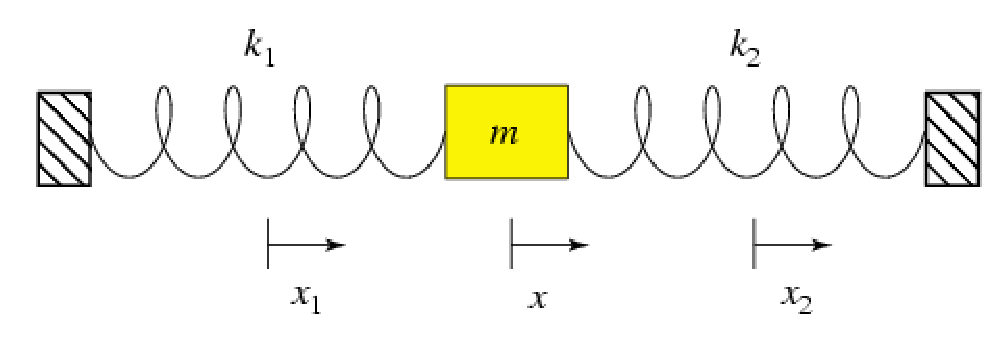
\includegraphics[height=3
cm]{./images/mass_2spring.eps}}
 \caption{An idealized system with a mass moving under the action of 2
   springs}
\label{fig:mass_2springs}
\end{figure}

In ideal condition, air resistance and internal friction of the
springs are neglected. For a small displacement $x$, there is an
elastic restoring force on the spring, i.e. the force, in the opposite
direction from the displacement, trying to restore the spring to its
equilibrium state. Thus, the equation of motion becomes
\begin{equation}
  \label{eq:361}
  F=ma = -k_1x-k_2x = -(k_1+k_2)x
\end{equation}
with $k_1>0,k_2>0$ are the spring constants (stiff springs have large
$k_i$;  soft springs have small $k_i$). This is aka {\bf Hooke's law} and it
holds as long as $x$ remains below the spring's elastic limit.

The {\it effective spring constant} of the system is
$k_{eff}=k_1+k_2$. Thus, setting $\sqrt{\frac{k}{m}}=\omega_0$ as the
{\bf angular oscillation frequency}, and the spring's motion is the
differential equation of a {\it simple harmonic oscillator} (in its
so-called {\bf canonical form}) is
\begin{equation}
  \label{eq:363}
  \ddot{x} + \omega^2_0 x = 0
\end{equation}
whose \textcolor{red}{analytical solution} is
\begin{equation}
  \label{eq:364}
  \begin{split}
    \dot{x} &=-\omega_0K\sin(\omega_0t + \alpha)\\
    x &= A\cos(\omega_0t) + B\sin(\omega_0t) = Kcos(\omega_ot+\alpha)
  \end{split}
\end{equation}
with $K=\sqrt{A^2+B^2}, \alpha = \arctan(-\frac{B}{A})$.


\subsection{-- properties}

{\bf REVIEW}: A simple oscillating oscillator has these 3 following
properties:
\begin{enumerate}
\item motion is periodic
\item motion is about an equilibrium point at which no net force
  acting on the system
\item restoring force is proportional to and oppositely directed to
  the displacement. 
\end{enumerate}

The restriction of this result is that (1) the displacement should be
small, (2) the number of oscillation is limited (as the energy is
assumed to be conserved). We also need the initial conditions
($x(0),\dot{x}(0)$) in order to solve eq.~\eqref{eq:364} completely.

\subsection{-- trajectory}

Based on the analytical solution, the displacement $x$ is represented
by a ``sinusoidal curve'' characterized by 3 quantities ($K$: maximum
deviation (amplitude of the displacement), $\omega_o$: angular
frequency (number of oscillations during $2\pi$ seconds; $\alpha$:
phase angle), as shown in Fig.~\ref{fig:sinusoidal_curve}.

\begin{figure}[hbt]
 \centerline{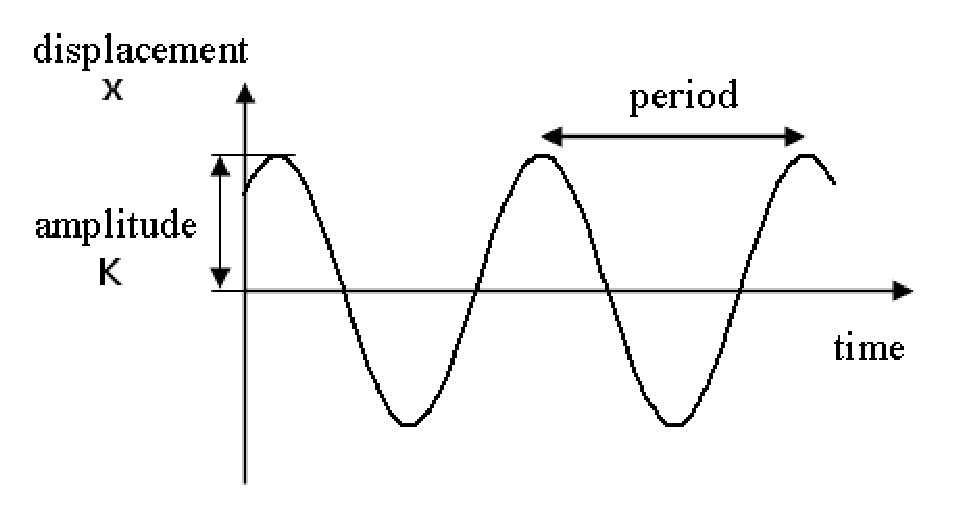
\includegraphics[height=4cm]{./images/sinusoidal_curve.eps}}
\caption{The simple harmonic oscillator with $\alpha=-\pi/2$}
\label{fig:sinusoidal_curve}
\end{figure}

$K$ is completely determined by the initial conditions, $\omega_0$ is
determined by the nature of the system. 

\subsection[Simplest non-linear oscillator with damping: (van der Pol)]{Simplest
non-linear oscillator with damping: (van der Pol):
$ \ddot{x} + \mu (x^2-1) \dot{x} + x = 0\; ; \; \mu>0$}
\label{sec:simplest-nonlinear-oscill}
\label{sec:van-der-Pol-equation}

The example in Sect.\ref{sec:simplest-linear-oscill} possesses a permanent and
symmetric oscillations. In real world, there is no permanent oscillations, i.e.
every oscillation has a {\it damping constant} expressing the decay of the
oscillation after disturbance, e.g. the friction term. % Only the slightest
%disturbance can
% also move thing, except in well-known physical medium, e.g. in vacuum tubes.
It means the first-order term of $x$ needs to be added, i.e. $\dot{x}$, to
represent the friction effect, Fig.\ref{fig:van-der-Pol-damping-oscillation}.

\begin{figure}[hbt]
  \centerline{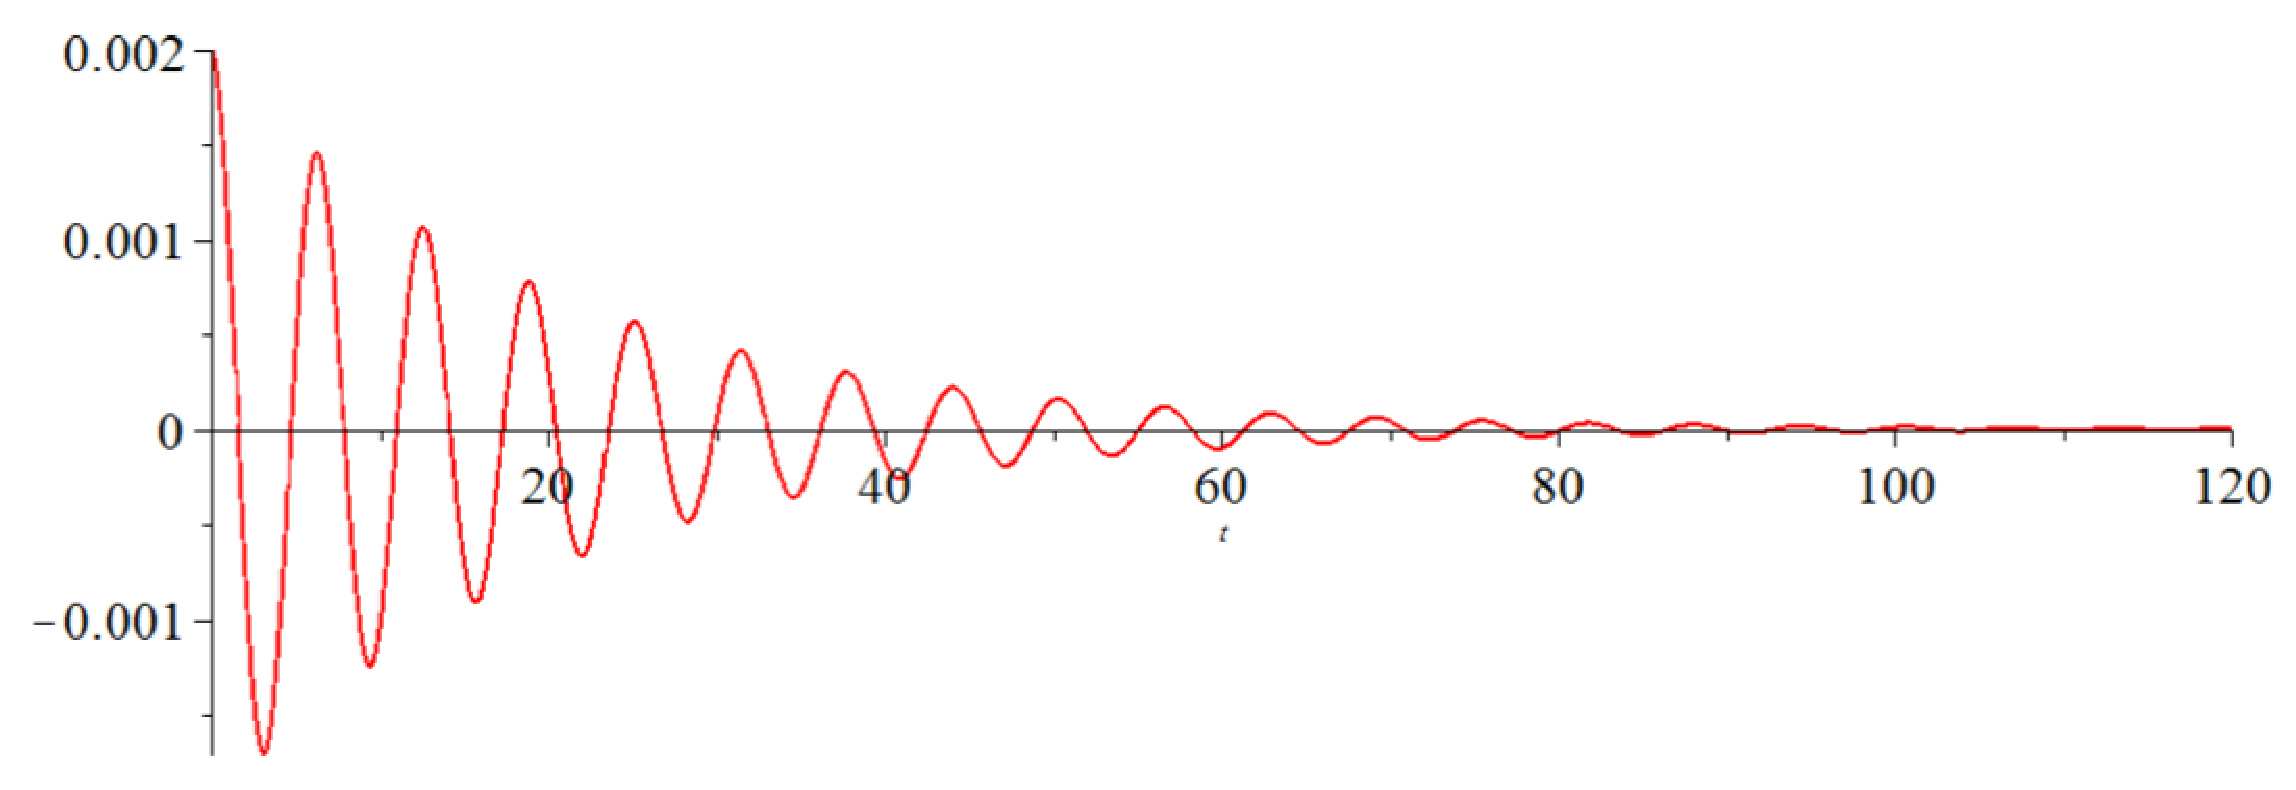
\includegraphics[height=3cm,
    angle=0]{./images/van-der-Pol-damping-oscillation.eps}}
\caption{van der Pol damping oscillation with $b = -0.1$}
\label{fig:van-der-Pol-damping-oscillation}
\end{figure}



\begin{framed}

In our scenario, we are mainly interested in homogeneous systems
(Sect.\ref{sec:homogeneous-system})
\begin{equation}
  \label{eq:371}
  a\ddot{x}+b\dot{x}+cx=0, \text{with } abc\ne 0
\end{equation}
($b$: friction
coefficient\footnote{friction force per unit of velocity}). 
\end{framed}

Here, we examine a second-order linear equation with friction term added
\begin{equation}
  \label{eq:78}
   \ddot{x}+k\dot{x}+x=0
\end{equation}
with $k$ is called the {\it damping constant}\footnote{damping is any
  effect that tends to reduce the amplitude of oscillations in an
  oscillatory system}. 

To convert it to the non-linear system, \citep{vanderPol1926} replaced the
damping constant by a damping coefficient which depends quadratically on $x$.
\begin{equation}
  \label{eq:372}
  \ddot{x} + \mu (x^2-1) \dot{x} + x = 0\; ; \; \mu>0
\end{equation}
Here, $k=\mu(x^2-1)$ is the nonlinear {\it damping coefficient} (friction
or resistance) with $\mu>0$. 

Eq.\ref{eq:372} is a second order ODE with cubic nonlinearity and is the
simplest non-linear equation whose solution is periodic, This is called the {\bf
van der Pol equation}.
This is a stable oscillations, which he called {\it relaxation-oscillations}, or
now known as {\it limit cycles} (i.e. at least one trajectory spiral into it
when time approaches infinity).

\subsection{-- van der Pol: systems of two first-order linear ODEs}
\label{sec:van-der-Pol-2-ODEs}

One way to solve the van der Pol equation is to convert to a system of
first-order
ODEs\footnote{\url{http://math.fullerton.edu/mathews/n2003/VanDerPolMod.html}}
(the method is described in Sect.~\ref{sec:linear-system}).
\begin{equation}
  \label{eq:580}
  \begin{split}
    \dot{x} &= y \\
    \dot{y} &= -x - \mu(x^2-1)y
  \end{split}
\end{equation}

The system enters limit cycle (Sect.\ref{sec:limit-cycle}) when $\mu > 0$, as
shown in Fig.\ref{fig:vanderPol_harmonic-oscillation}. When $\mu=0$,
Fig.\ref{fig:van_der_Pol}(A), the system is a simple harmonic oscillator.

\begin{figure}[hbt]
  \centerline{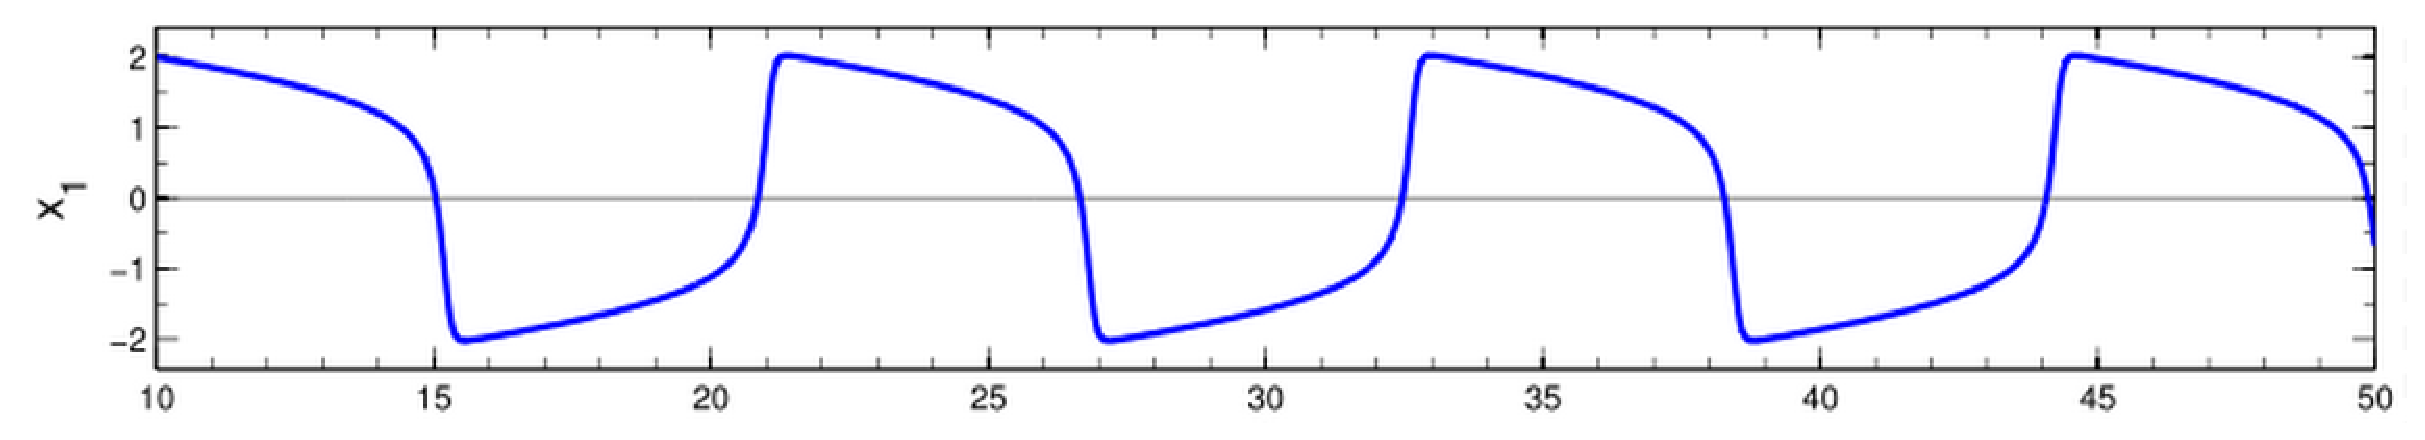
\includegraphics[height=2cm,
    angle=0]{./images/vanderPol_harmonic-oscillation.eps}}
  \caption{Relaxation-oscillation without external forcing, $\mu=5$}
  \label{fig:vanderPol_harmonic-oscillation}
\end{figure}

If we set $\mathbf{z}=(x,y)$, then we can re-write the system in the form 
\begin{equation}
  \label{eq:581}
  \dot{\mathbf{z}} = \mathbf{f}(\mathbf{z})
\end{equation}
This can be solved easily using any available numerical package
(Sect.\ref{sec:packages}) with a given initial value $\mathbf{z}_0$.
Some of the solution is given in Fig.~\ref{fig:van_der_Pol}. This will
be reviewed in next sections.

\begin{figure}[hbt]
  \centerline{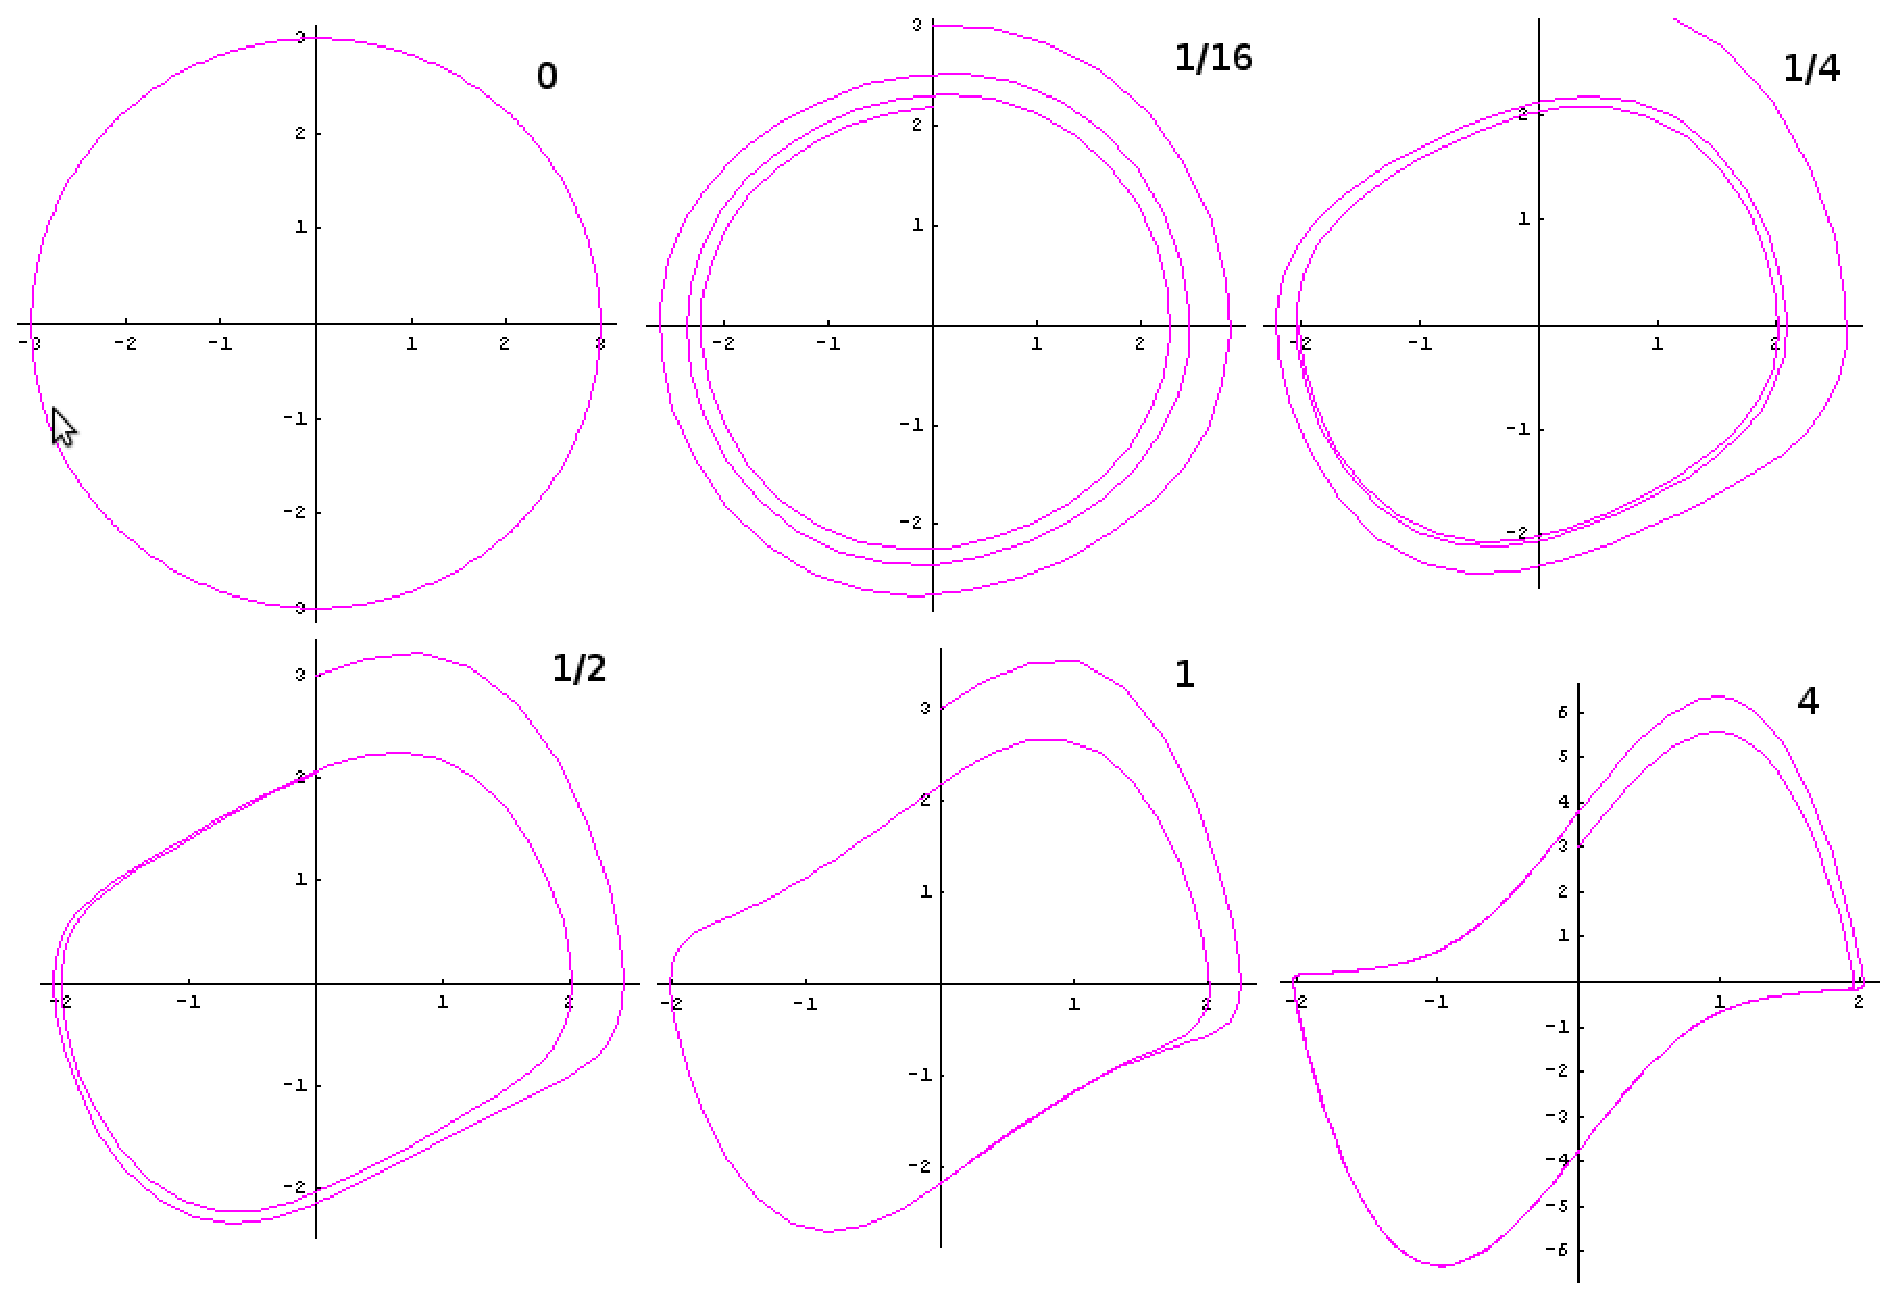
\includegraphics[height=6cm,
    angle=0]{./images/van_der_Pol.eps}}
  \caption{Solution of the van der Pol equation with different values
    of $\mu$. (A) when $\mu=0$ the system become linear oscillator; (B-F)
    dampled oscillation with different shapes}
\label{fig:van_der_Pol}
\end{figure}

{\bf Example}: $\mu=1/16$, $\mathbf{z}_0 = (x_0,y_0)=(0,3)$. In the
interval $[a,b]$, we divide into $m$ segments, thus the time step is
$ dt=h=\frac{b-a}{m}$. 
\begin{verbatim}
RungeKutta_2D[a, b, x0, y0, m]
  h = (b-a)/m
  T = table[ a+(j-1)*h, {j=1,m+1} ]
  Z = table[ {x0,y0}, {j=1,m+1} ]

  For j=1, j<=m, j++
     k1 = h*F[T[j], Z[j]]
     k2 = h*F[T[j] + h/2, Z[j]+k1/2]
     k3 = h*F[T[j] + h/2, Z[j]+k2/2]
     k4 = h*F[T[j] + h,   Z[j]+k3]
     Z(i+1) = Z(i) + 1/6(k1 + 2*k2 + 2*k3 + k4) 
  EndFor
  return Z
\end{verbatim}

\subsection{Other forms of van der Pol equations}


Using Lienard's transformation
\begin{eqnarray}
y = x - \frac{1}{3}x^3 - \frac{1}{\mu}\dot{x} \\
\end{eqnarray}
then the van der Pol equation become
\begin{eqnarray*}
\label{eq:vanderPol-Lienard}
    \dot{x} &&= \mu \left( x-\frac{1}{3}x^3 - y \right) \\
    \dot{y} &&= \frac{1}{\mu}x
\end{eqnarray*}

\subsection{forced van der Pol: chaotic behavior}
\label{sec:forced-van-der-Pol-equation}

\begin{mdframed}

HISTORY: Van der Pol (in 1927) did the experiments with oscillations in the
vacuum tube triode circuit and concluded that all initial conditions converged
to the same periodic orbit of finite amplitude.
Since this behavior is different from the behavior of solutions of linear 
equations, van der Pol proposed a nonlinear differential equation \ref{eq:372}.
This is called {\it unforced Van der Pol equation}.

When study the case $\mu \gg 1$, he discovered the importance of what we call
{\bf relaxation oscillations}. Then, he proposed the second form that includes a
periodic forcing term (Sect.\ref{sec:forced-van-der-Pol-equation})
\begin{equation}
\ddot{x} + \mu (x^2-1) \dot{x} + x = a \sin(\omega t)\; ; \; \mu>0
\end{equation}

It has become the prototype for systems with self-excited limit cycle
oscillations. The Fitzhugh-Nagumo equation is a planar vector field that extends
the van der Pol equation as a model for action potentials of neurons
(Sect.\ref{sec:fitzh-nagumo-model}).

\end{mdframed}

A 'force' term can also be added to create forced van der Pol oscillator
\begin{equation}
  \ddot{x} + \mu (x^2-1) \dot{x} + x + F(t) = 0\; ; \; \mu>0
\end{equation}
With a constant force, there is no chaotic evolution. Yet, chaotic behavior
occur when using an sinosuidal forcing: $F(t)=-A\sin(\omega t)$, as shown in
Fig.\ref{fig:vanderPol_sinosuidalforce}.

\begin{figure}[hbt]
  \centerline{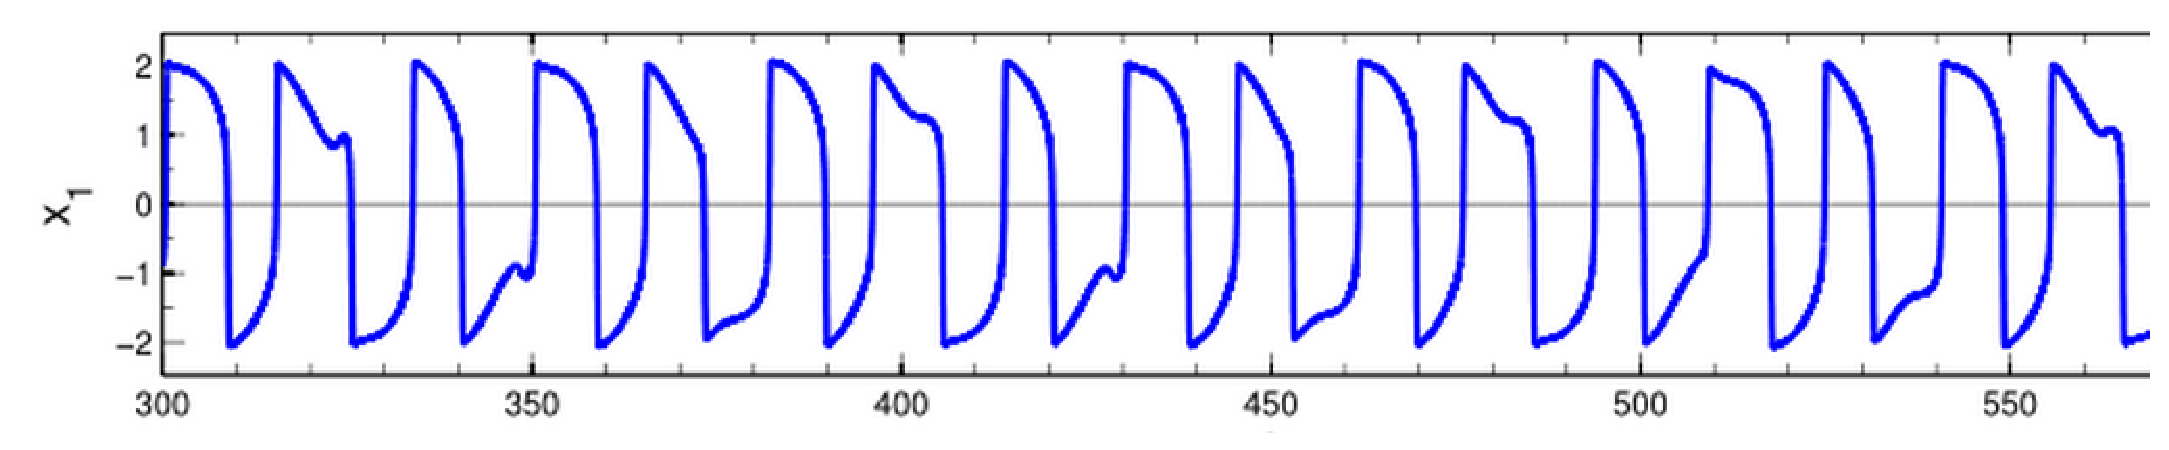
\includegraphics[height=2cm,
    angle=0]{./images/vanderPol_sinosuidalforce.eps}}
  \caption{Chaotic behavior when using sinosuidal force: A=1.2,
  $\omega=2\pi/10$, and damping coefficient $\mu=8.53$}
  \label{fig:vanderPol_sinosuidalforce}
\end{figure}


\section{System of first-order ODEs}
\label{sec:linear-system}

A first-order system is the one in which the highest order of derivative is
first-order. Any system of higher order, can be converted to first-order system
by adding more variables, as shown in the example of van der Pol equation
(Sect.\ref{sec:van-der-Pol-2-ODEs}).
% Any non-linear homogeneous autonomous system of any order of derivatives can
% be converted to a set of linear first-order derivatives.
This is very important as mathematicians have developed many method to solve
first-order system (Sect.\ref{sec:packages}). In first-order linear system, the
left-hand size is normally the first-order derivative.

{\bf Example}: Consider the second-order system in eq.~\eqref{eq:363}
\begin{equation}
  \label{eq:366}
  \ddot{x} + \omega_0^2x=0
\end{equation}
we don't need the analytical solution to analyze the system.  The
procedure is as follows:

\begin{enumerate}
\item A new variable is defined: $y=\dot{x}$. Thus the system is now
  described as
  \begin{equation}
    \label{eq:367}
    \begin{split}
      \frac{dx}{dt} &= y \\
      \frac{dy}{dt} &= -\omega^2_0x
    \end{split}
  \end{equation}
\end{enumerate}

\begin{framed}

A general 2D first-order system is
\begin{equation}
  \label{eq:592}
  \begin{split}
    \frac{dx}{dt} &= f(x,y,t) \\
    \frac{dy}{dt} &= g(x,y,t)
  \end{split}  
\end{equation}
\end{framed}

A general form of a 2D linear first-order system is
\begin{equation}
  \label{eq:593}
  \begin{split}
    \frac{dx}{dt} &= ax+by+r_1(t) \\
    \frac{dy}{dt} &= cx+dy+r_2(t)
  \end{split}    
\end{equation}
There are two cases
\begin{itemize}
\item $a,b,c,d$ are constants, then the system is called a system with
  constant coefficient.
\item $a,b,c,d$; each can be a function of $t$.
\end{itemize}
In any cases, if $r_i(t)=0$ then we have a linear homogeneous system.

\begin{framed}

When $x,y$ are the only dependent variables, and $t$ is independent variable in
the system, $t$ can be removed from $f(\cdot),g(\cdot)$ by introducing a new
dependent variable $z=t$. Then, such system is called {\bf autonomous} (read
Sect.~\ref{sec:auton-syst-vs}). It's also important to know that most
multivariate first-order ODE system, especially in nature, are non-linear.
\end{framed}

{\bf IMPORTANT}: A good habbit is always write the dependent variables
in the right hand size in the order that they appear, e.g. if $x$ in
the first equation, then $x$ is always written first. This will help us in
writing the matrix form to solve the system using eigenvector-eigenvalues
method. Below is an example of BAD habbit
\begin{equation*}
  \begin{split}
    \frac{dx}{dt} &= by+ax+r_1(t) \\
    \frac{dy}{dt} &= dy+cx+r_2(t)
  \end{split}    
\end{equation*}

\subsection{Coupled vs. Uncoupled system}
\label{sec:coupled-vs.-uncoupled}

In a set of ODE, if solving one equation is independent of the other,
then the system is uncoupled, eq.~\eqref{eq:634}
\begin{equation}
  \label{eq:634}
  \begin{split}
    \dot{x} &= ax^3 \\
    \dot{y} &= -y + y^2
  \end{split}
\end{equation}

Otherwise, if solving one equation depends on the others, the system is coupled.
They are more important as most physical systems are coupled.
Solving uncoupled system is easier than coupled system. All the system we study
in the previous section are the coupled
system\footnote{\url{http://string.howard.edu/~tristan/Research/CuplPDEs.htm}}.

Implicit numerical methods are often used to solved coupled system.

\subsection{Autonomous system vs. Non-autonomous system}
\label{sec:auton-syst-vs}

Given a physical system, {\bf stability analysis} is critical to the
system.
\textcolor{blue}{The use of {\it autonomous systems} is essential to
  stability analysis.}
An autonomous system is a system of ODE that doesn't depend on the
independent variable, e.g. the time. Thus, autonomous system has the
rate of change is independent of time, while a non-autonomous system
has a time-dependent rate.

For an autonomous system,
\begin{enumerate}
\item the trajectory of the system cannot cross itself, except it is a
  closed trajectory. This is not true in non-autonomous system.
\item there always exists a trajectory through any point
\item if the functions on the right hand side,
  e.g. $f(\cdot)=0,g(\cdot=0)$, are smooth functions, then we get unique
  solution. % Given that the trajectory through a single point is
  % unique, then if the two systems go through a single point at
  % different time, then the two trajectories are translation (in time)
  % to each other.
\end{enumerate}

\subsection{-- Autonomous system}
\label{sec:autonomous-system}

Examples of autonomous system:
\begin{itemize}
\item first-order autonomous system
  \begin{eqnarray}
    \label{eq:537}
    \frac{dx}{dt} = f(x)
  \end{eqnarray}
\item second-order autonomous system
  \begin{eqnarray}
    \label{eq:538}
    \frac{d^2x}{dt^2} = f(x,\dot{x})
  \end{eqnarray}
\item ...
\end{itemize}

Practically, an {\bf autonomous system} is represented as a set
homogeneous first-order ODEs in which the time appear at the
differential $dt$ only, i.e. the right hand-side of every equations
has no time variable $t$. Example:

\begin{itemize}
\item Univariate: $\frac{d}{dt}x(t) = \dot{x} = f(x)$ with $x$ is the
  time-variant quantity.

\item Bivariate: 
  \begin{equation}
    \label{eq:99}
    \begin{split}
      \frac{d}{dt}x(t) = \dot{x} = f(x,y) \\
      \frac{d}{dt}y(t) = \dot{y} = g(x,y)
    \end{split}
  \end{equation}
with $x,y$ are time-variant quantities.

\item $n$-variable: $\dot{x_i} = f_i(x_1,x_2,\dots,x_n)$,
  $j=\overline{1,\dots,n}$, where $x_i$ are time-variant quantities. 
\end{itemize}
In summary, the vector form of an autonomous system is
$\dot{\mathbf{x}}=\mathbf{f(x)}$. % The use of autonomous systems is
% essential to stability analysis.

Historically, autonomous systems first appeared in descriptions of
physical processes with a finite number DOFs. We can imagine that an
autonomous system is a mathematical model that describes the
characteristics of a real world system that we want to design.

\subsection{-- Nonautonomous system}
\label{sec:nonautonomous-system}


Example of non-autonomous system
\begin{itemize}
\item $\frac{dx}{dt} = f(x,t)$
\end{itemize}

A {\bf non-autonomous system}, when represented in the mathematical
form as a set of ODEs, this set of ODEs should has at least one
equation whose right-side formula contains the time $t$, e.g.
$\dot{\mathbf{x}}=\mathbf{f(x},t)$. 


However, a $n$-dimensional
non-autonomous system can be casted to a $(n+1)$-dimensional
autonomous system by introducing a new unknown function $x_{n+1}=t$.
Example: $\ddot{x} = F(x,\dot{x})$ is recast into standard form by
introducing a new variable $v=\dot{x}$.

% In the previous example, the analytical solution for $x$ could be
% obtained. However, in many cases, it is impossible or costly to obtain
% it. How can we analyze such systems? - There is a method to do that.
\textcolor{red}{The main point is that any system, can be converted to
  the autonomous form}.

\section{Phase plane (X vs. t, or X vs. Y)}
\label{sec:phase-plane}

A degree of freedom is the minimum number of coordinates required to specify the
position of a particle or system of particles. In equation, the system has one
degree of freedom (DOF), when the state of the system is determined by a pair of
$(x(t), \dot{x}(t))$.  Here, we focus on a system of 2 dependent variables or
the system with two degrees of freedom.

In a system represented by a second-order ODE, it can be converted to a system
of first-order ODE by introducing a new dependent variable $y=\dot{x}$, as
described in Sect.~\ref{sec:linear-system}. This is the main theme of the
discussion topic in the whole-chapter. The solution of this system of ODE, e.g.
$(x(t),y(t))$, for a given set of parameters values, when plotted in the
x,y-plane, we obtain the so-called {\bf phase curve} (level curves or (phase)
{\it trajectories}). In Fig.\ref{fig:van_der_Pol}, each plot is a phase curve.
The coordinate system in which the phase curve is plotted is called {\bf phase
plane}. If we extend it to $n$-dimensional space, phase plane is called {\bf
phase space} instead. \textcolor{red}{As state variables were called {\it phase
variables} back in the old days, it is where the name {\it phase plane} comes
from}.

For a given set of parameters' values (and an initial condition $(x_0,y_0)$),
the time course of the system is drawn into a single trajectory. In other words,
the phase curve show the trajectory of the system over time. The motion along
that curve is known as {\bf phase flow} in literature (as the motion on the
phase curve bears a close relation to the flow concept in hydrodynamics).  The
point M(x,y) is referred to as a {\bf representative point} (or phase point) of
the system.  In summary, it's a visualization display of the system. The
velocity $(\dot{x}, \dot{y})$ of the point $M$ is called {\bf phase velocity}
(IMPORTANT: this is not the velocity of the system). The phase velocity is
denoted as $v=(\dot{x},\dot{y})$.

When multiple phase curves (corresponding to different set of parameter's value
and initial conditions) are plot on the same phase plane, the set of all phase
curves is called the {\bf phase portrait}.  The interesting fact is that by
looking at the phase portrait, one may state several important properties of the
system.
\textcolor{red}{Luckily, there are tools that can do this task for us}. The
technique to interpret the phase plane is called {\bf phase plane analysis}
(Sect.\ref{sec:phase-plane-analysis}).
\begin{enumerate}
\item XPPAUT
\item PPtool (Matlab)
\end{enumerate}

{\bf Example}: Let's examine the previous oscillator under the new
view point of a phase plane (using
\textcolor{red}{analytical solution})
\begin{equation}
  \label{eq:362}
  \begin{split}
    x &= K\cos(\omega_0t+\alpha)\\
    y &= \dot{x}= K\sin(\omega_0t+\alpha)
  \end{split}
\end{equation}
Then, by eliminating the time, we have the form of an ellipse.
\begin{equation}
  \label{eq:373}
  \begin{split}
    \frac{x^2}{K_0^2}+\frac{y^2}{K_0^2\omega_0^2} = 1
  \end{split}
\end{equation}
As $K$ is determined by the initial condition of the system, eq.~\eqref{eq:373}
indeed defines a family of ellipses. 


\begin{enumerate}
\item The ellipse passing through the origin is merely the point
  itself.

\item Each ellipse correspond to a given condition and these ellipses
  are concentric.

\item Let's examine a single path, the motion of $M$ is always
  clockwise since the positive of $y$ corresponding to the increase in
  the value of $x$, and the negative of $y$ corresponding to the
  decrease in the value of $y$.

\item The phase velocity is tangent to the trajectory, points in the
  direction of motion and the length (magnitude) is the phase speed
  \begin{equation}
    \label{eq:365}
    \begin{split}
          v
          &= (v_x, v_y) = (\dot{x},\dot{y})= (-K\omega_0\sin(\omega_0t+\alpha),-K\omega^2_0\cos(\omega_0t+\alpha))
          \\
          |v|&=K\omega_0\sqrt{\sin^2(\omega_0t+\alpha)+\omega^2_0\cos^2(\omega_0t+\alpha)}
    \end{split}
  \end{equation}
The phase velocity is always between $K\omega_0$ and $K\omega^2_0$.
\end{enumerate}

\subsection{Isoclines}
\label{sec:isoclines}

In the phase plane of an autonomous system, the set of points having
the same phase velocity (slope), say $\beta$, forms a curve calls
{\bf isoclines}. In our example of a simple harmonic oscillator, each
isocline is a straight line passing through the origin.

The slope is also $\frac{dy}{dx}$. Consider an explicit example in
which with the slope $\beta$, the time is eliminated and the following
equation is solved
\begin{equation}
  \label{eq:369}
  \frac{dy}{dx} = -\omega_0^2\frac{x}{y}  = \beta
\end{equation}
then
\begin{eqnarray*}
  y=\sigma x \\
  \sigma= -\frac{\omega_0^2}{\beta}
\end{eqnarray*}

\begin{figure}[hbt]
  \centerline{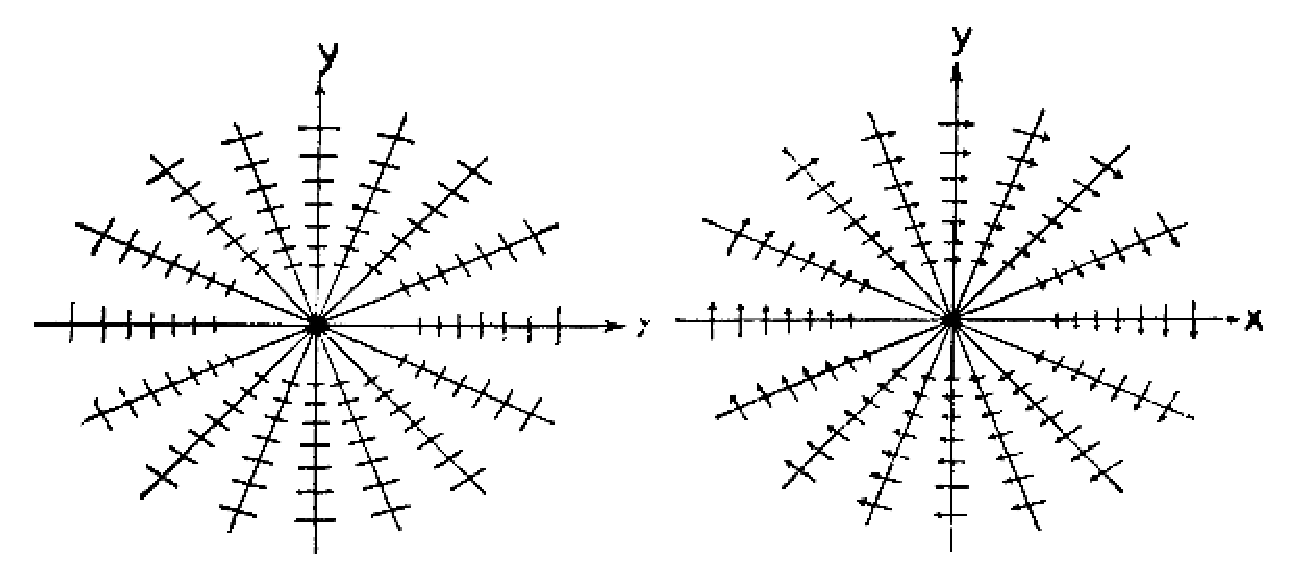
\includegraphics[height=5cm]{./images/isoclines.eps}}
  \caption{The isoclines of the simple harmonic oscillator}
  \label{fig:isocline_sho}
\end{figure}

From this, we can expect the isocline to go through the origin.  What
if we want to know the general form of the path?  By transforming the
problem into the new form
\begin{equation}
  \label{eq:374}
  ydy + \omega_0^2xdx = 0
\end{equation}
and taking the integral, we have
\begin{equation}
  \label{eq:375}
  y^2 + \omega_0^2x^2 = C
\end{equation}
If we set $C=K$, then we get a similar form to the analytical solution
of $x$ as shown in eq.~\eqref{eq:373}.

To tells us the direction of motion and the corresponding phase
velocity, the arrow is added and the length of each arrow indicates
the magnitude of the phase velocity, as shown in
Fig.~\ref{fig:isocline_sho}.




\subsection{Nullclines}
\label{sec:nullclines}

Consider a two-variable autonomous system, 
\begin{equation}
  \label{eq:350}
  \left\{
    \begin{array}{cc}
      \frac{dx}{dt} = f(x,y)\\
      \frac{dy}{dt} = g(x,y)
    \end{array}
  \right.
\end{equation}
The x-{\bf nullcline} is the set of point so that
$\frac{dx}{dt}=0$. Geometrically, these are the point where the
vectors are straight up or straight down. Similar definition for
$y$-nullcline. 
\textcolor{red}{A nullcline is also known as zero-growth isocline}.

Algebraically, we can find x-nullclines by solving $f(x,y)=0$; and
$y$-nullcline by solving $g(x,y)=0$. 

For phase plane analysis, we need to draw two nullclines,
$x$-nullcline and $y$-nullcline on x-y plane. The set of all (x,y) on
the $x$-nullcline make the system doesn't change w.r.t. $x$. Similarly,
the set of all (x,y) on the $y$-nullcline make the system doesn't
change w.r.t. $y$. When the two nullclines intersect, the intersection
points are the point when the system doesn't change at all. This is
known as {\bf fixed-point} or {\bf singular point}. We'll study it
next section.


\subsection{Singular points (fixed-point) and critical point}
\label{sec:singular-points}


For a given initial condition, the system will have a unique
trajectory path. However, there are points at which the velocity is
zero
\begin{equation}
  \label{eq:583}
  \dot{x}=0, \dot{y} = 0
\end{equation}
These points never change and are called {\bf singular points}
(fixed-point). The trajectory path through such a point is reduced to
a single point. As we can see in Fig.~\ref{fig:van_der_Pol}, singular
points occur when $\mu=1/2, 1$.  The singular point is the intersect
of two nullclines: one x-nullcline and one y-nullcline.

The concept of {\bf critical point} is larger than
{\bf singular points}.  A critical point can be (1) a point at which
  the function cannot be differentiable, (2) singular point.
% In the example of a system of simple harmonic oscillation, the only
% singular point is the origin $(0,0)$.  
The singular points correspond to states of {\it equilibrium}. In many
cases, but not all, the reverted statement,'' the equilibrium states
is the singular points'', is true. We will study about equilibrium
shortly.


\subsection{Stability of equilibrium}
\label{sec:stab-equil}

An equilibrium state is the state at which there is no motion (no
change). So, we consider the two equilibrium states of the pendulum,
one when it is at (a) position and one at (b) position, both with
initial velocity zero, as shown in Fig.~\ref{fig:pendulum}.  The only
difference is that the previous state is stable, while the other one
is unstable. The reason is that at the stable equilibrium, if the
pendulum perturb/displace from its stable position a little bit, it's
still going back to the stable position. This doesn't happen with
unstable equilibrium.

The point at which the system remain stable equilibrium is called
{\bf stable point}. There are also other types of points.  For more
information about stability, read next Chapter,
sect.~\ref{sec:stability}.

\begin{figure}[hbt]
  \centerline{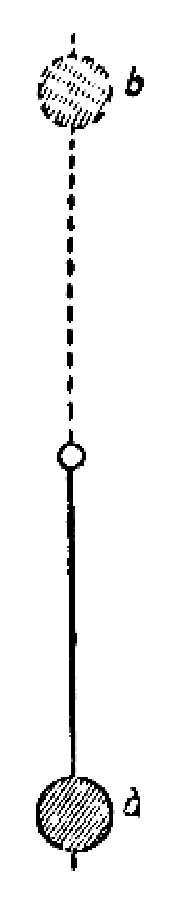
\includegraphics[height=5cm]{./images/pendulum.eps}}
  \caption{The pendulum}
  \label{fig:pendulum}
\end{figure}

Also, an equilibrium state is called {\it ``conditionally''} stable if
we eliminate a certain class of displacements, e.g. it won't stable if
the displacement is in horizontal direction. Next, the question is how
do we define ``near'' or ``in the vicinity of''?  To examine if an
equilibrium state is stable or not, {\bf phase plane} is utilized. In
phase plane, the singular points are equilibrium states.  So, this is
the definition:

\begin{itemize}
\item A state of equilibrium is stable whenever given any region
  $\epsilon$ containing that state, there is always a smaller region
  $\delta(\epsilon)$ in $\epsilon$ such that any motion starting in
  $\delta(\epsilon)$ remain in $\epsilon$. 

\item A state of equilibrium is unstable whenever given any region
  $\epsilon$ containing that state, there is always a point $M$ within
  such that a motion starting from $M$ leaves $\epsilon$
\end{itemize}

\begin{figure}[hbt]
  \centerline{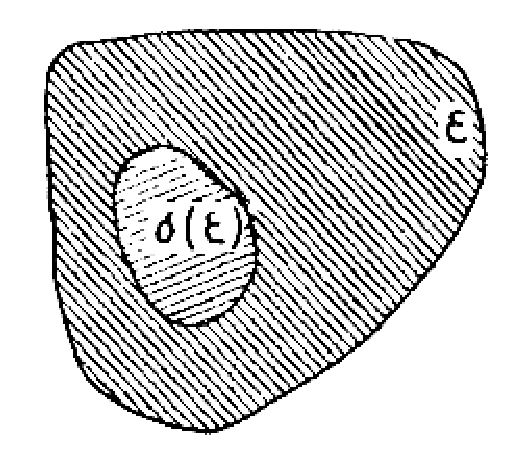
\includegraphics[height=5cm]{./images/perturb_vicinity.eps}}
  \caption{A perturb in motion}
  \label{fig:perturb}
\end{figure}

There is also another definition is called
{\bf stability according to Lyapunov}~\cite{andronow1949osci}. It is
said that if you can find a region from which the system start off, if
it remains in this region, then the system is stable, in the sense of
Lyapunov. Lyapunov stability is weak, as it doesn't require
$\mathbf{x}(t)$ to converge to $\mathbf{x}_e$ as $t\rightarrow
\infty$. 

\section{Phase plane analysis}
\label{sec:phase-plane-analysis}

The introduction is given in the beginning of the chapter
\ref{chap:phase-plane-analysis}. Here, we describes in details.

In 1D, the coordinate of the phase plane is $\dot{X}$ vs. $X$.
In 2D, the coordinate of the phase plane is $X$ vs. $Y$. Most of the time, to
perform phase analysis, the system is autonomous
(Sect.\ref{sec:autonomous-system}), with two dependent variables represented in
first-order ODE form.
\begin{equation}
  \label{eq:678}
  \begin{split}
    \dot{x} = f(x,y)\\
    \dot{y} = g(x,y)
  \end{split}
\end{equation} 

\begin{framed}

For systems of higher dimension (Sect.\ref{sec:fitzh-nagumo-model}), fast
time-scale and low time-scale analysis can be performed first to know which
parameter have a faster kinetics and slow kinetics. When we study two dependent
variables of slowest kinetics, we just assign other variables to their
steady-state values, i.e. the derivative is zero. Another way for dimension
reduction is {\bf dimensional analysis} technique which make variable unitless
and also reduce the number of variables also.
\end{framed}

\begin{enumerate}
  \item By using {\bf isoclines} (Sect.\ref{sec:isoclines}), it can tells when the
dependent variables has the same rate of changes ($\dot{x},\dot{y}$). With the
arrow, it can tell the direction of the changes (increasing or decreasing).
  
  \item There are situations when the rate of changes is zero. This can tell by
  looking at the x-nullcline or y-nullcline on the x-y phase plane. The
  intersection of the x-nullclines and y-nullclines gives are the points at
  which the rate of changes is zero. They are called {\bf fixed-point} or
  singular point.
  It represents the state at which the system has reached the {\it equilibrium}
  condition. However, the equilibrium can be stable or unstable.
   
\end{enumerate}
However, there's a more powerful method to analyze the system, without needing
to find the trajectory of the system for every set of parameter's values and
initial condition. The method is {\bf bifurcation theory} (Appendix
\ref{chap:bifurcation-theory}).

\subsection{Solving first-order linear ODEs - eigenvalues method}
\label{sec:eigenvalues-method}
\label{sec:characteristic-function}

Now, we consider again a 2D first-order ODE. Let's take a practical
example: We put an egg in the bath with temperature $T_e(t)$. The egg
has its yolk with temperature $T_1(t)$, while the temperature of the
white part of the egg is $T_2(t)$. 
\begin{equation}
  \label{eq:594}
  \left\{
    \begin{array}{ll}
      \frac{dT_1}{dt} &= a(T2-T1) = -aT_1 + aT_2\\
      \frac{dT_2}{dt} &= a(T1-T2) + b(T_e-T_2) = aT_1 - (a+b)T_2 + bT_e
    \end{array}
  \right.
\end{equation}
with $a$ is the heat conductance between the yolk and the white part,
$b$ is the heat conductance between the white part and the bath. The
bath temperature is assumed to be constant. 

To make it a homogeneous system, we assume $T_e=0$. But, instead of
using $T_1,T_2$, we define $x=T_1, y=T_2$. We also set the
conductivity as $a=2, b=3$. 

\begin{equation}
  \label{eq:595}
  \begin{split}
    \dot{x} &= -2x + 2y \\
    \dot{y} &= 2x - 5y
  \end{split}
\end{equation}

Of course, we can easily find out the general solution, is
\begin{equation}
  \label{eq:596}
  \begin{split}
    x &= c_1e^-t - c_2 e^{-6t} \\
    y &= c_1/2e^{-t} - 2c_2 e^{-6t}
  \end{split}
\end{equation}
with 2 arbitrary constants. However, in practice, a widely use method
is {\bf eigenvalues method}. 

We write a matrix whose component is the differential of the
appropriate variable.
\begin{equation}
  \label{eq:597}
  \left(
    \begin{array}{c}
      x \\ y
    \end{array}
  \right)' =   \left(
    \begin{array}{cc}
      -2  & 2 \\ 2 & -5
    \end{array}
  \right)    \left(
    \begin{array}{c}
      x \\ y
    \end{array}
  \right)
\end{equation}
with 
\begin{equation*}
  \left(
    \begin{array}{cc}
      -2  & 2 \\ 2 & -5
    \end{array}
  \right)   = \left(
    \begin{array}{cc}
      f_x  & f_y \\ g_x & g_y
    \end{array}
  \right)   
\end{equation*}

If we look back the analytical solution, we can write it in the form
\begin{equation}
  \label{eq:598}
  \left(
    \begin{array}{c}
      x \\ y
    \end{array}
  \right) = c_1  \left(
    \begin{array}{c}
      1 \\ 1/2
    \end{array}
  \right) e^{-t} + c_2  \left(
    \begin{array}{c}
      1 \\ -2
    \end{array}
  \right) e^{-6t}
\end{equation}
The question is how we can derive eq.~\eqref{eq:598} from
eq.~\eqref{eq:597}?

{\bf NOTE 1}: This is a first-order linear ODE, remember that in 1D,
the solution is exponential decay function; so for the 2D, the guest
solution can be
\begin{eqnarray*}
  x = a_1e^{\lambda_1t} \\
  y = a_2e^{\lambda_2t} 
\end{eqnarray*}
However, this doesn't work. The reason is that we can see from the
analytical solution, in the two components of the solution, they both
use the same exponential factor. Thus, a better guess is
\begin{equation*}
  \left(
    \begin{array}{c}
      x \\ y
    \end{array}
  \right)  =  \left(
    \begin{array}{c}
      a_1 \\ a_2
    \end{array}
  \right) e^{\lambda t}
\end{equation*}
So, now we can reduce the calculus problem (with derivative) to
algebra problem, with matrix handling. 
\begin{equation}
  \label{eq:599}
  \lambda \left(
    \begin{array}{c}
      a_1 \\ a_2
    \end{array}
  \right) e^{\lambda t} =   \left(
    \begin{array}{cc}
      -2  & 2 \\ 2 & -5
    \end{array}
  \right)   
  \left(
    \begin{array}{c}
      a_1 \\ a_2
    \end{array}
  \right) e^{\lambda t}
\end{equation}
Here, we have two equations with 3 unknown variables
\begin{eqnarray*}
  \lambda a_1 = -2a_1 + 2a_2 \\
  \lambda a_2 = 2a_1 - 5a_2
\end{eqnarray*}
This is non-linear as we have multiply two unknown variables. However,
if we temporarily consider $\lambda$ as a constant, we now have a
perfect two equations with 2 unknown and the system is homogeneous
also. 
\begin{equation}
  \label{eq:600}
  \begin{split}
    (-2-\lambda) a_1 + 2a_2 = 0 \\
    2 a_1 - (5+\lambda)a_2 = 0
  \end{split}
\end{equation}
Of course, we don't want the trivial solution $(0,0)$ as it doesn't
give any information. In the case of non-trivial solution
(i.e. non-zero). The system has non-trivial solution if and only if
the determinant of the matrix is zero.
\begin{equation}
  \label{eq:601}
  \left|
    \begin{array}{cc}
      -2-\lambda & 2 \\
      2& -5-\lambda
    \end{array}
  \right| = 0
\end{equation}
or 
\begin{eqnarray*}
  \lambda^2 + 7\lambda + 6 = 0
\end{eqnarray*}
which is called the {\bf characteristic equation}. There are two
solutions $\lambda=-1, \lambda=-6$. 
\begin{itemize}
\item $\lambda=-1$
  \begin{equation}
    \label{eq:602}
    \begin{split}
      -a_1 + 2a_2 = 0 \\
      2a_1 - 4a_2 = 0
    \end{split}
  \end{equation}
\item $\lambda=-6$
  \begin{equation}
    \label{eq:602}
    \begin{split}
      4a_1 + 2a_2 = 0 \\
      2a_1 + a_2 = 0
    \end{split}
  \end{equation}
\end{itemize}
{\bf IMPORTANT}: For a value of $\lambda$, one equation must be a
multiple of the other, the reason is that we can never have a unique
pair of $(a_1,a_2,\lambda)$. So, if we fix $\lambda$, $a_1,a_2$ will
vary. 

Set one to unit value, e.g. $a_1=1$, then we can find $a_2$ in both
cases, $a_2 = 1/2, a_2 = -2$. Finally, the solution of the original
system is
\begin{equation}
  \label{eq:603}
  \tilde{c_1}   \left(
    \begin{array}{c}
      1 \\ 1/2
    \end{array}
  \right) e^{-t} + \tilde{c_2}  \left(
    \begin{array}{c}
      1 \\ -2
    \end{array}
  \right) e^{-6t}
\end{equation}
$\lambda$ is called the {\bf eigenvalue} of the matrix. 

\begin{framed}

\textcolor{red}{Solving first-order autonomous system, one important
remark is that the solution is in the form of exponential function of
$t$. That's why we'll see that in many mathematical model of a
physiological system, exponential terms are widely used.}
\end{framed}

{\bf SUMMARY}: In general, a linear system can be represented as
$\mathbf{\dot{x} = Ax}$, the two eigenvalues are similar to eq.~\eqref{eq:89}.
Phase-plane behavior is depending on these two eigenvalues. The eigenvalue will
be complex if $4\det(\mathbf{A}) > (tr(\mathbf{A})^2)$.
Two diagrams to help remembering are given in Fig.\ref{fig:dynamic_behavior}
(linear-system) and Fig.\ref{fig:phase-plane_behavior} (non-linear).

\begin{itemize}
\item Real $\lambda_i$:
  \begin{itemize}
    \item Sink (stable nodes) : $Re(\lambda_1)<0, Re(\lambda_2)<0$
    \item Source (unstable nodes) :$Re(\lambda_1)>0, Re(\lambda_2)>0$
    \item Saddle (unstable) : $Re(\lambda_1)<0, Re(\lambda_2)>0$
  \end{itemize}
\item Complex $\lambda_i$: 
  \begin{itemize}
    \item Focus (Spirals) : $\lambda_1$ and $\lambda_2$ are complex conjugate. If
  $Re(\lambda_1)<0$, then stable focus. If $\lambda_1>0$, then
  unstable focus.  
    \item Center (Vortex): imaginary eigenvalues (e.g. $\pm 4i$).
  \end{itemize}
\end{itemize}

\begin{figure}[htb]
  \centerline{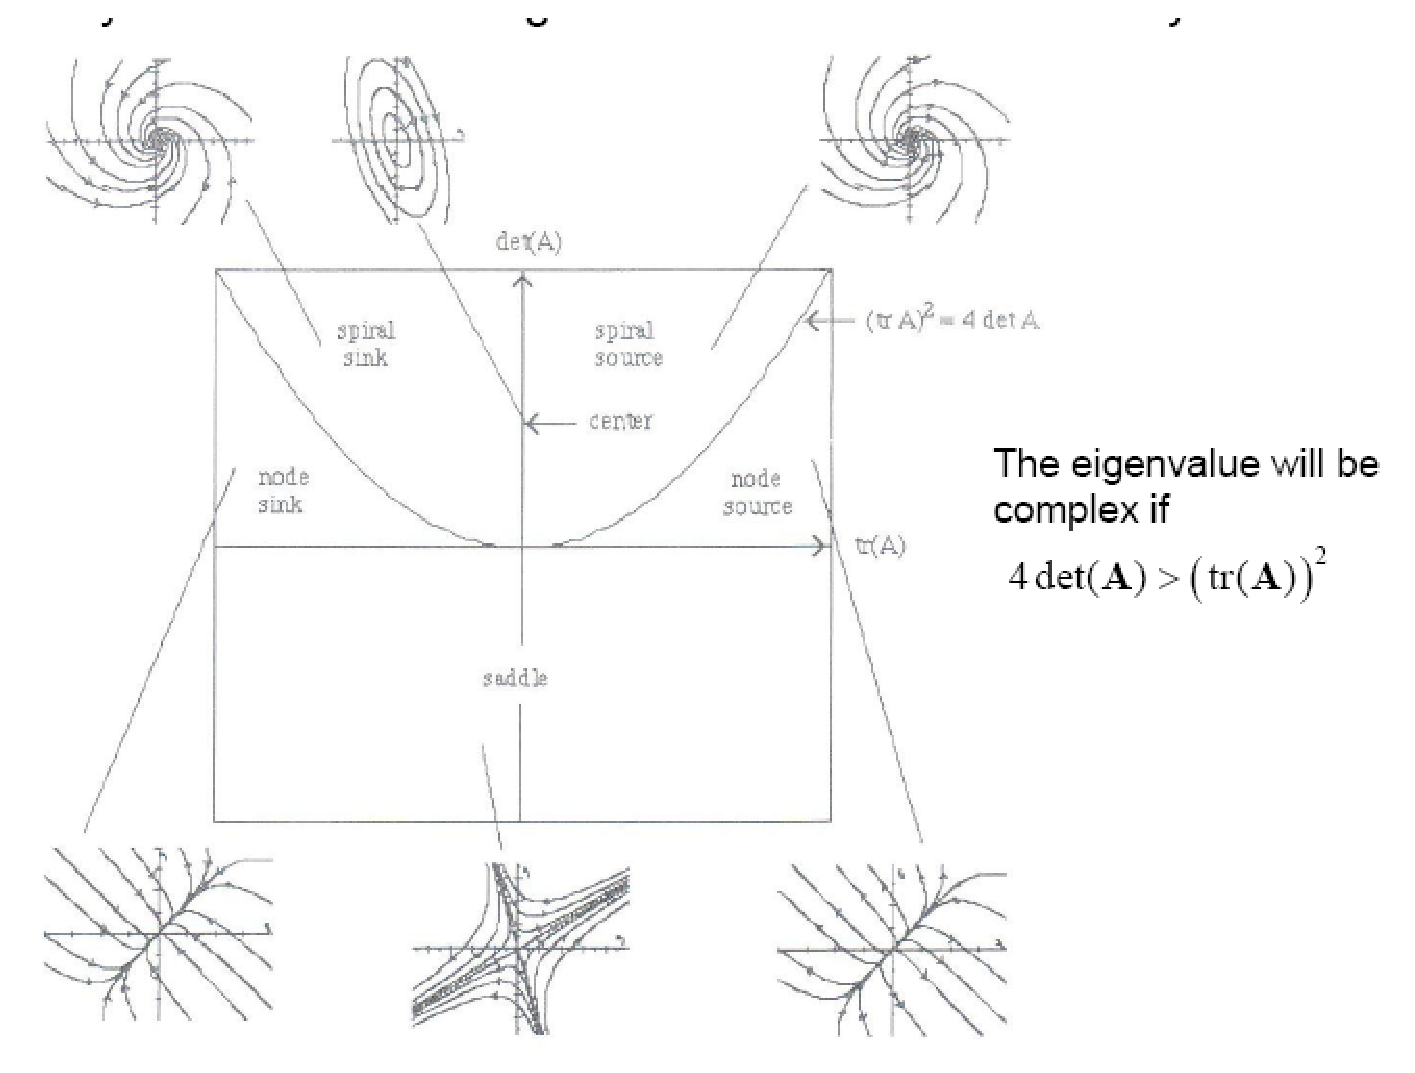
\includegraphics[height=7cm]{./images/dynamic_behavior_diagram.eps}}
  \caption{The diagram to help analyze behavior of a linear system}\label{fig:dynamic_behavior}
\end{figure}


\subsection{Damped system}
\label{sec:damped-system}


Based on the oscillation in eq. \eqref{eq:363}, the homogeneous
nonlinear oscillator, as described in eq.~\eqref{eq:371}, now can be
written as

\begin{equation}
  \label{eq:376}
  \ddot{x}+2h\dot{x}+\omega_0^2x=0
\end{equation}
with $h$ is the damping coefficient. $h$ is the controlling parameter
that define the ``qualitative'' aspect of the system. Using phase plane
analsyis, we can easily investigate the topological
structure change of the system when $h$ is changed by clicking a point in the
plot to add a new trajectory using phase plane analysis. 

\subsubsection{Analytical solution}
\label{sec:analytical-solution-damped-system}

We consider the situation when the analytical solution is
obtainable. Solving it, we obtained an exponentially damped
oscillation, as shown in Fig.~\ref{fig:damped_osc}.
\begin{equation}
  \label{eq:377}
  \begin{split}
    \dot{x} &= -K e^{-ht}(h\cos(\omega_1t + \alpha)+\omega_1\sin(\omega_1t+\alpha)) \\
    x &= e^{-ht}(A\cos(\omega_1t)+B\sin(\omega_1t))=Ke^{-ht}\cos(\omega_1t+\alpha) \\
  \end{split}
\end{equation}
with $K=\sqrt{A^2+B^2}, \alpha=\arctan(-\frac{B}{A})$.

This is not periodic, however, the time
between two consecutive zeros of $x$ is $T_1=2\pi/\omega_1$ and is
called {\it ``conditional period''}. As the amplitude changes after
each conditional period, the amplitude is called conditional
amplitude. The time for $x$ to decrease a factor of $1/e$ (about 63\%)
is called the {\it time constant} and is equal to $1/h$. As the value
of $h$ is depending the choice of time unit, a unitless measure of
damping is proposed, called {\bf logarithmic decrement}, $d=T_1h$
(i.e. the ratio of displacement one period apart).
\begin{enumerate}
\item $1/d$ is the number of ``conditional period'' after which the
  amplitude decreases to $1/e$ of its value.
\item what we have discussed is only valid for ``linear friction'';
  otherwise, the notion of logarithmic decrement loses its meaning.
\item conditional period and logarithmic decrement is determined by
  the properties of the system
\item amplitude and phase are determined by the initial condition.
\end{enumerate}

\begin{figure}[hbt]
  \centerline{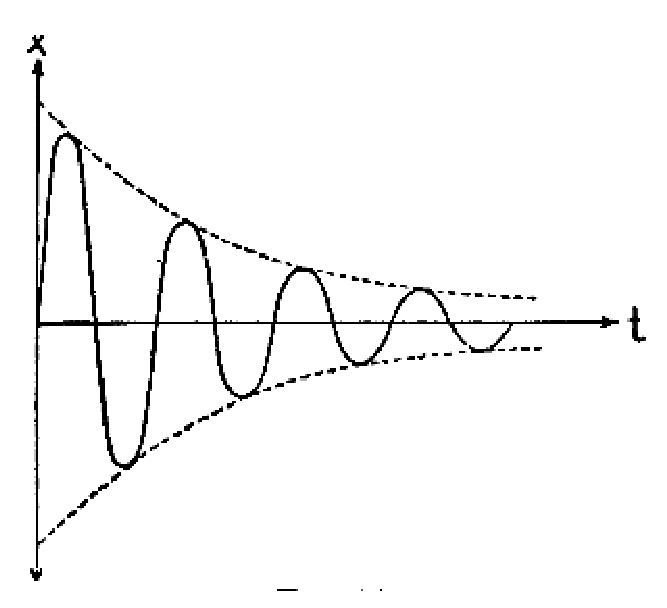
\includegraphics[height=5cm]{./images/damped_oscillator.eps}}
  \caption{Damped oscillator}
  \label{fig:damped_osc}
\end{figure}

\subsubsection{A damped system in phase plane}
\label{sec:damped-system-phase}

The damped system, in the phase plane, has the phase portrait as a
family of spirals with an asymptotic point at the origin, as shown in
Fig.~\ref{fig:spiral_damped}.

\begin{figure}[hbt]
  \centerline{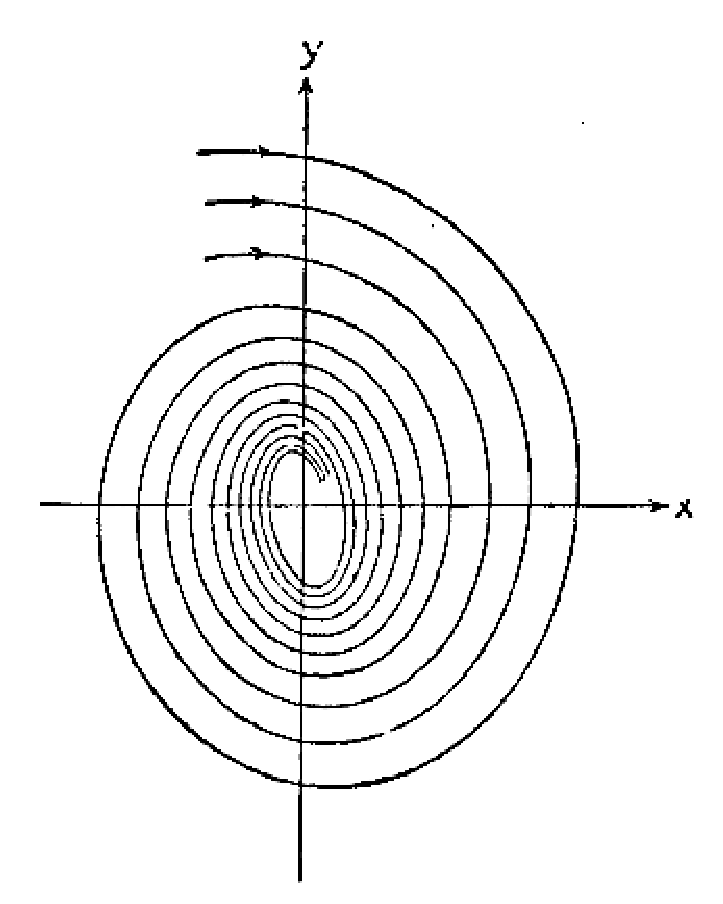
\includegraphics[height=5cm]{./images/spiral_damped_system.eps}}
  \caption{A phase portrait of the damped system, showing a family of
    spirals with an asymptotic point as origin}
  \label{fig:spiral_damped}
\end{figure}

This can be achieved by applying a linear transformation to the
original equations.
\begin{equation}
  \label{eq:378}
  \begin{split}
    u &= \omega_1x=\omega_1Ke^{-ht}\cos(\omega_1t+\alpha) \\
    v &= hx+y =  -\omega_1Ke^{-ht}\sin(\omega_1t+\alpha) \\
  \end{split}  
\end{equation}
Then, we map it to the Polar coordinate, as shown in Fig. with
\begin{equation}
  \label{eq:379}
  \begin{split}
    r&=\sqrt{u^2+v^2}=\omega_1Ke^{-ht}\\
    \psi&=\omega_1t+\alpha
  \end{split}
\end{equation}

\begin{figure}[hbt]
  \centerline{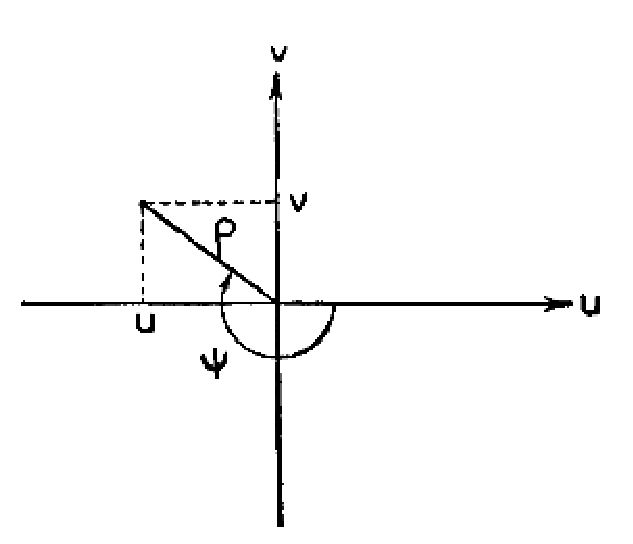
\includegraphics[height=5cm]{./images/polar_damped_sys.eps}}
  \caption{The damped oscillator in polar coordinate system}
  \label{fig:polar_damped}
\end{figure}
The point $M$ move in clockwise with angular angle $\psi$ and the
radius $r$ decreases exponentially and asymptotically to the
origin. Thus, it is known as {\bf logarithmic spirals}. The common
asymptotic point of a family of concentric spirals here is called a
{\bf focus}.

Likewise, the question next we have to answer is whether the focus is
stable or not. We will talk in detail for the case of numerical
solution. 


\subsubsection{Numerical solution}
\label{sec:numerical-solution-1}

In general cases, analytical solutions are often unavailable. Thus we
need a way to analyze the system without knowing its analytical
solution. A new variable $y$ is defined
\begin{equation}
  \label{eq:380}
  \begin{split}
    \frac{dx}{dt} &= y \\
    \frac{dy}{dt} &= -2hy - \omega_0^2x
  \end{split}
\end{equation}
Again, we need to eliminate the time parameter from the system
\begin{equation}
  \label{eq:381}
  \frac{dy}{dx} = \frac{-2hy - \omega_0^2x}{y}
\end{equation}
Again, this equation defines the set of point $M(x,y)$ having the same
phase velocity $\beta$, i.e. it defines certain field of tangent on the phase
plane. If we give $\beta$ to a sufficiently large number of values
($h$ and $\omega_0$ being fixed by the system), then we will get a set
of isoclines, as shown in Fig. \ref{fig:damped_isocline}.

\begin{figure}[hbt]
  \centerline{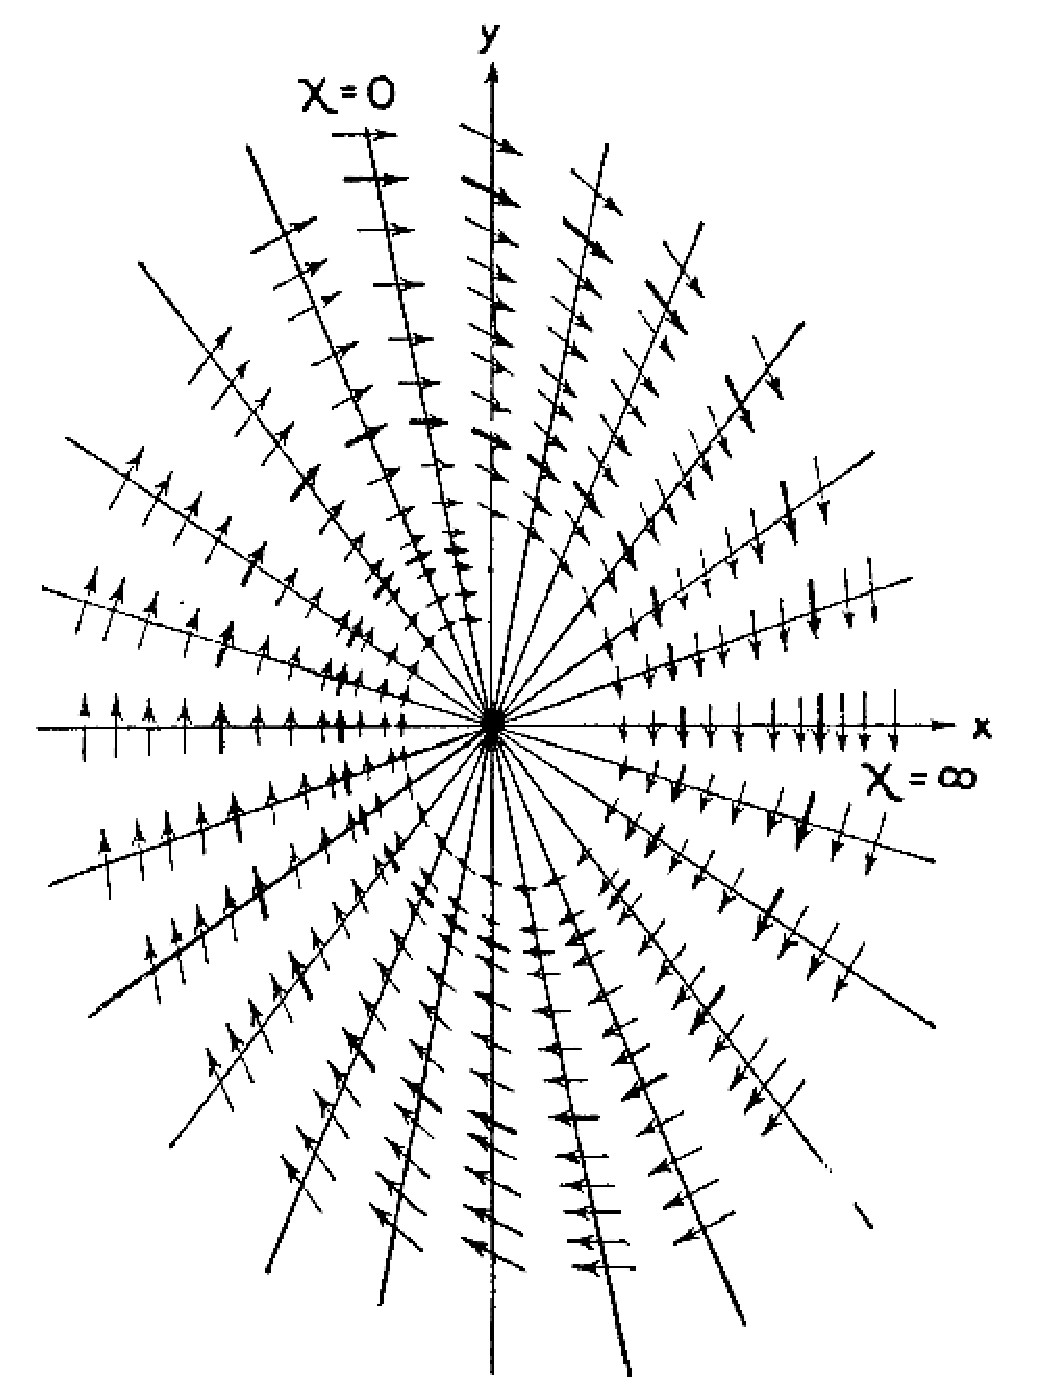
\includegraphics[height=5cm]{./images/damped_isoclines.eps}}
  \caption{Isoclines of a damped oscillator}
  \label{fig:damped_isocline}
\end{figure}


Numerical analysis returns approximated solutions for free parameters
(state variables) in a dynamical system. In order to solve the set of
ODEs, it is required to have a set of initial values. Thus the problem
is called {\it initial values problem}. It means that the solutions
were dependent upon the initial conditions. As a matter of fact, for a
complete understanding of the response characteristic of the system,
we still need some methods to study the general behaviors of a
non-linear system, i.e. without spending the time to compute the time
evolution of the system when different initial conditions are
given. 

\subsection{Phase plane plot}
\label{sec:phase-plane-plot}


% A phase plane plot is drawn on a plane with axes are one state
% variable versus the other state variable where each curve is based on
% a different initial condition, as shown in
% Fig.~\ref{fig:phase-plane_plot}.

\begin{figure}[hbt]
 \centerline{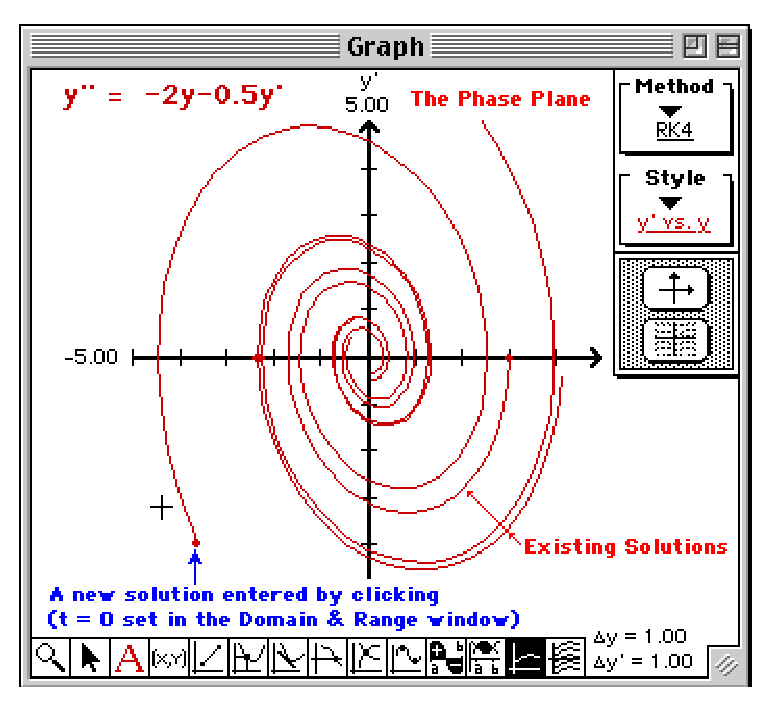
\includegraphics[height=6cm]{./images/phaseplane_plot.eps}}
\caption{An example of phase plant plot\footnote{\url{http://www2.umassd.edu/temath/TEMATH2/Tutorial/SolvingDiffEqns.html}}}
\label{fig:phaseplane_plot}
\end{figure}

% {\bf Knowledge base}: Suppose that $u$ is the x-axis and $v$ is the
% y-axis, the $u,v$-plane is called {\bf phase plane}, or phase space in
% general. And the curve, associated with a given initial condition is
% called a {\it trajectory} (or {\it phase-plane trajectory} or
% orbit). 

Such graphical plot, in general, transmits more information and make
more effective to readers than numeric values and text.
\textcolor{red}{Phase plane analysis is applicable to systems with two
  free parameters only}.
For 1 free parameter, we use {\bf phase-point analysis}.
% . In this method, the time element has
% been removed, i.e. there is no time involvement in the phase space

\subsection{Phase-point analysis}
\label{sec:phase-point-analysis}

We examine first-order homogeneous ODE.
\begin{equation}
  \label{eq:667}
  \frac{dc}{dt} = j - kc
\end{equation}
or 
\begin{equation}
  \label{eq:669}
  \frac{dc}{dt} = \frac{c_{ss}-c}{\tau}
\end{equation}
with 
\begin{eqnarray*}
  c_{ss} = j/k \\
  \tau = 1/k
\end{eqnarray*}

COPY 3 figures of stable, unstable from CSHL notes.


\subsection{Phase plane analysis on 2D linear system}
\label{sec:phase-plane-analysis-1}

Even though the phase plane analysis is mainly used to study the
behavior of non-linear system, a good starting point to comprehends
this method is by applying it for linear systems. In a linear system,
there is only a single steady state solution.

{\bf Example 1}:
\begin{equation}
  \label{eq:106}
  \begin{split}
    \begin{array}{c}
          \dot{x_1} = -x_1 \\
    \dot{x_2} = -4x_2
    \end{array}
\Rightarrow 
\begin{array}{c}
  x_1(t) = x_1(0) \exp(-t) \\
  x_2(t) = x_2(0) \exp(-4t)
\end{array}
  \end{split}
\end{equation}
Now, we will use phase-plane plot for different initial condition
$(x_1(0),x_2(0))$, Fig.\ref{fig:saddle_stable}.

\begin{lstlisting}
x1.0 = c(-4,-2,1,3)
x2.0 = c(-3,-1,2,4)

t = seq(0,5,0.1)

func_x1 = function(x1.0, t) {x1.0 * exp(-t)}

x1 = outer(x1.0, t, FUN=func_x1)

func_x2 = function(x2.0, t) {x2.0 * exp(-4*t)}

x2 = outer(x2.0, t, FUN=func_x2)

limit = c(-4,4)
line = c(1,2,3)
par(ann=F)
for (i in 1:length(x1[,1])) {
  for (j in 1:length(x2[,1])) {
    plot(x1[i,], x2[j, ], type="l", xlim=limit, 
               ylim=limit, lty=line[1])
    par(new=T, ann=F)
  }
}
points(0,0,col='red')
\end{lstlisting}


In this system, they all converge to a fixed-point (0,0) which is a
stable point. As the phase curves has the shape of a sink, the fixed point is
called a {\bf saddle stable point} (sink stable node).

\begin{figure}[htb]
  \centerline{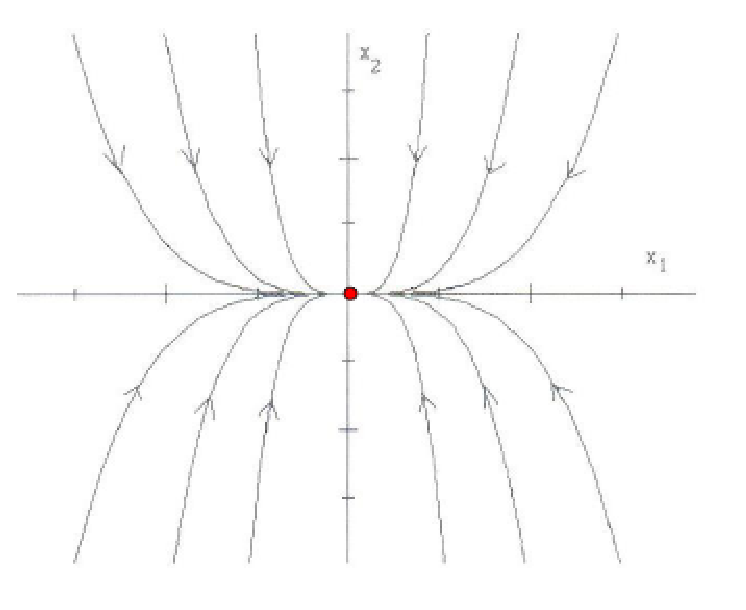
\includegraphics[height=5cm]{./images/stable_sink_node.eps}}
  \caption{The solution converge to (0,0) which is a stable fixed point}
  \label{fig:saddle_stable}
\end{figure}

{\bf Example 2}: We modify a little bit to the previous system, i.e. changing
the sign of the second parameter from -4 to 4.
\begin{equation}
  \label{eq:1061}
  \begin{split}
    \begin{array}{c}
          \dot{x_1} = -x_1 \\
    \dot{x_2} = 4x_2
    \end{array}
\Rightarrow 
\begin{array}{c}
  x_1(t) = x_1(0) \exp(-t) \\
  x_2(t) = x_2(0) \exp(4t)
\end{array}
  \end{split}
\end{equation}
Now, we will use phase-plane plot for different initial condition
$(x_1(0),x_2(0))$, Fig.\ref{fig:saddle_unstable}.

In this case, the trajectories converge to (0,0) only if $x_2(0) =
0$. Otherwise, the trajectories will always leave the origin. The
fixed point (0,0) is an unstable equilibrium of the system. 
\begin{lstlisting}
x1.0 = c(-4,-2,1,3)
x2.0 = c(-3,-1,0,2,4)

t = seq(0,5,0.1)

func_x1 = function(x1.0, t) {x1.0 * exp(-t)}

x1 = outer(x1.0, t, FUN=func_x1)

func_x2 = function(x2.0, t) {x2.0 * exp(4*t)}

x2 = outer(x2.0, t, FUN=func_x2)

xlimit = c(-5,5)
ylimit = c(-10,10)
line = c(1,2,3)
par(ann=F)
for (i in 1:length(x1[,1])) {
  for (j in 1:length(x2[,1])) {
    plot(x1[i,], x2[j, ], type="l", xlim=xlimit, 
          ylim=ylimit, lty=line[1])
    par(new=T, ann=F)
  }
}
points(0,0,col='red')
\end{lstlisting}
The $x_1$-axis represents a stable subspace, while $x_2$-axis
represents an unstable subspace. As the shape of the two subspaces
look like a saddle, the fixed point is called the {\bf saddle
unstable point}.
\begin{figure}[htb]
  \centerline{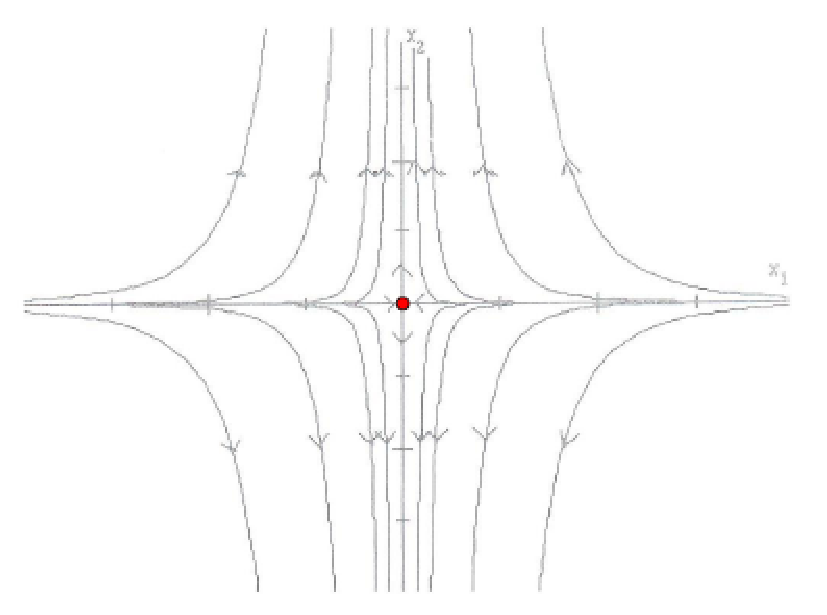
\includegraphics[height=5cm]{./images/saddle_point.eps}}
  \caption{The fixed point is unstable}\label{fig:saddle_unstable}
\end{figure}

{\bf Example 3}: This a more complicated linear system
\begin{equation}
  \label{eq:1062}
  \begin{split}
    \begin{array}{c}
          \dot{x_1} = 2x_1 + x_2 \\
    \dot{x_2} = 2x_1 - x_2
    \end{array}
\Rightarrow
\mathbf{\dot{x} = A.x}
\text{ with } \mathbf{A} = \left[
\begin{array}{cc}
  2 & 1 \\
  2 & -1 \\
\end{array}
\right]
  \end{split}
\end{equation}

To find out the fixed points for this system, you can use the method
described in sec. \ref{sec:singular-points}. The eigenvalues are
\begin{equation}
  \label{eq:107}
  \lambda_1 = -1.5616 , \lambda_2 = 2.5616
\end{equation}
and the eigenvectors are
\begin{equation}
  \label{eq:108}
  \xi_1 = \left[
    \begin{array}{c}
      0.2703 \\
      -0.9628
    \end{array}
    \right]
    ,
  \xi_2 = \left[
    \begin{array}{c}
     0.8719 \\
      0.4896
    \end{array}
    \right]
\end{equation}
The fixed point is still an unstable equilibrium solution and is
called {\bf source} unstable nodes.
\begin{figure}[htb]
  \centerline{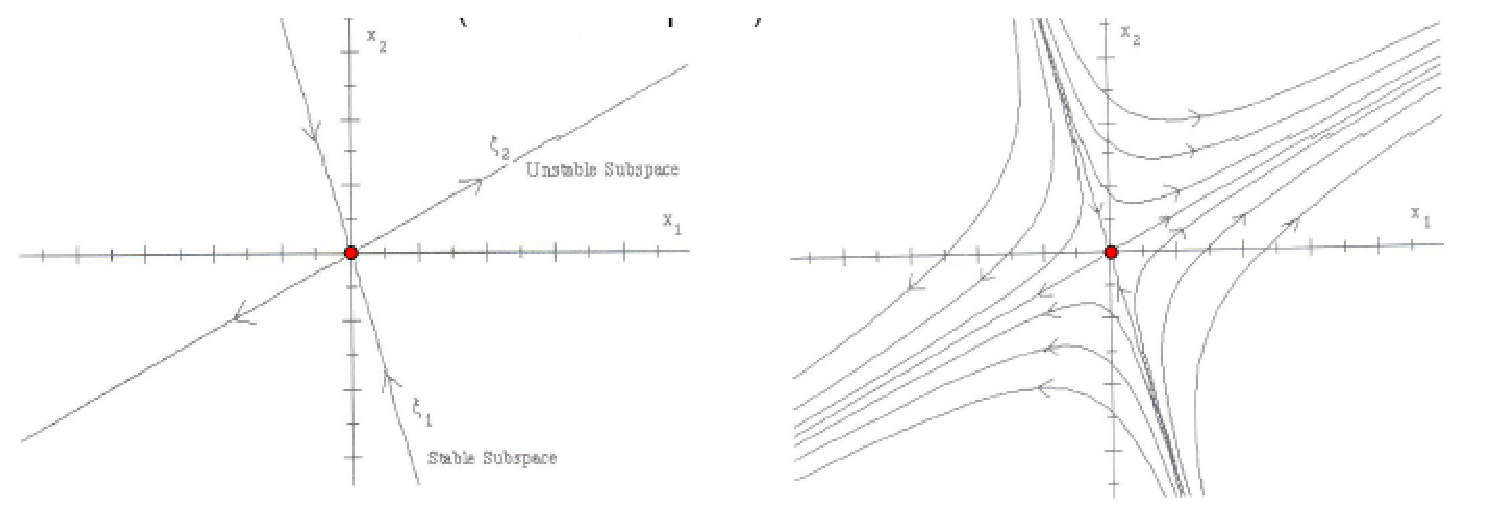
\includegraphics[height=5cm]{./images/unstable_subspace.eps}}
  \caption{The fixed point is unstable}\label{fig:unstable_subspace}
\end{figure}

{\bf Example 4:} Here, the situation is getting more complicated when
the eigenvalues are complex values. In this situation, the sign of the
real part of the eigenvalues is very important

\begin{equation}
  \label{eq:1063}
  \begin{split}
    \begin{array}{c}
          \dot{x_1} = x_1 + 2x_2 \\
    \dot{x_2} = -2x_1 + x_2
    \end{array}
\Rightarrow
\mathbf{\dot{x} = A.x}
\text{ with } \mathbf{A} = \left[
\begin{array}{cc}
  1 & 2 \\
  -2 & 1 \\
\end{array}
\right]
  \end{split}
\end{equation}

To find out the fixed points for this system, you can use the method
described in sec. \ref{sec:repr-dynam-syst}. The eigenvalues are
\begin{equation}
  \label{eq:1072}
  \lambda_1 = 1 \pm 2i
\end{equation}
(the eigenvectors are skipped)

The fixed point now is called an unstable {\bf spiral focus} as the
real part of the eigenvalues is positive.
\begin{figure}[htb]
  \centerline{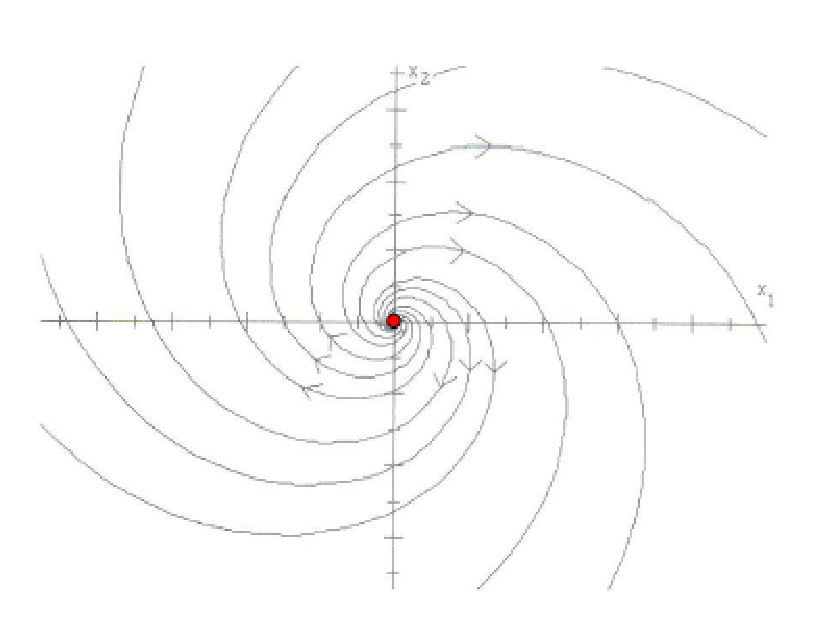
\includegraphics[height=5cm]{./images/unstable_spiral.eps}}
  \caption{The fixed point is an unstable spiral focus}\label{fig:unstable_spiral}
\end{figure}

{\bf Example 5:} Here, you will examine the case when the real part of
the eigenvalues is zero.

\begin{equation}
  \label{eq:1064}
  \begin{split}
    \begin{array}{c}
          \dot{x_1} = -x_1 - x_2 \\
    \dot{x_2} = 4x_1 + x_2
    \end{array}
\Rightarrow
\mathbf{\dot{x} = A.x}
\text{ with } \mathbf{A} = \left[
\begin{array}{cc}
  -1 & -1 \\
  4 & 1 \\
\end{array}
\right]
  \end{split}
\end{equation}

To find out the fixed points for this system, you can use the method
described in sec. \ref{sec:repr-dynam-syst}. The eigenvalues are
\begin{equation}
  \label{eq:1073}
  \lambda_1 = \pm 1.7231i
\end{equation}
(the eigenvectors are skipped)

As the real part of the eigenvalues is zero, there is a periodic
solution, with the equilibrium point is the {\bf center}.
\begin{figure}[htb]
  \centerline{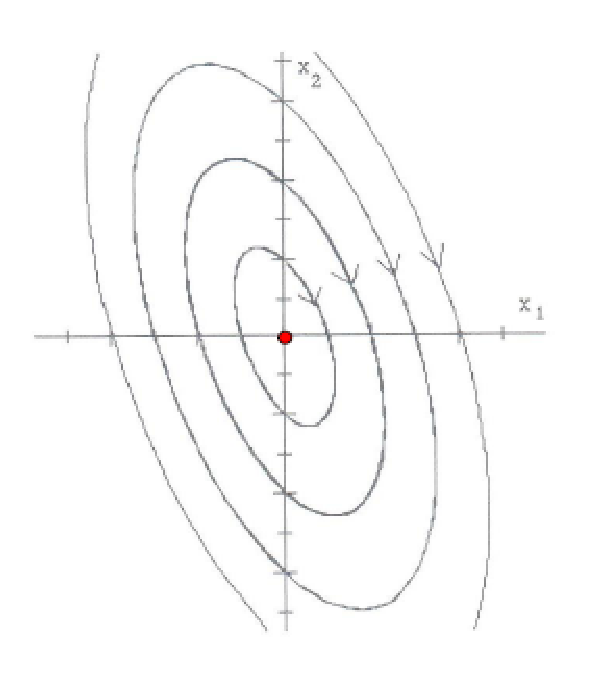
\includegraphics[height=5cm]{./images/center_fixed_point.eps}}
  \caption{The fixed point is a center of the phase curve}\label{fig:center_fixed_point}
\end{figure}


\begin{figure}[htb]
  \centerline{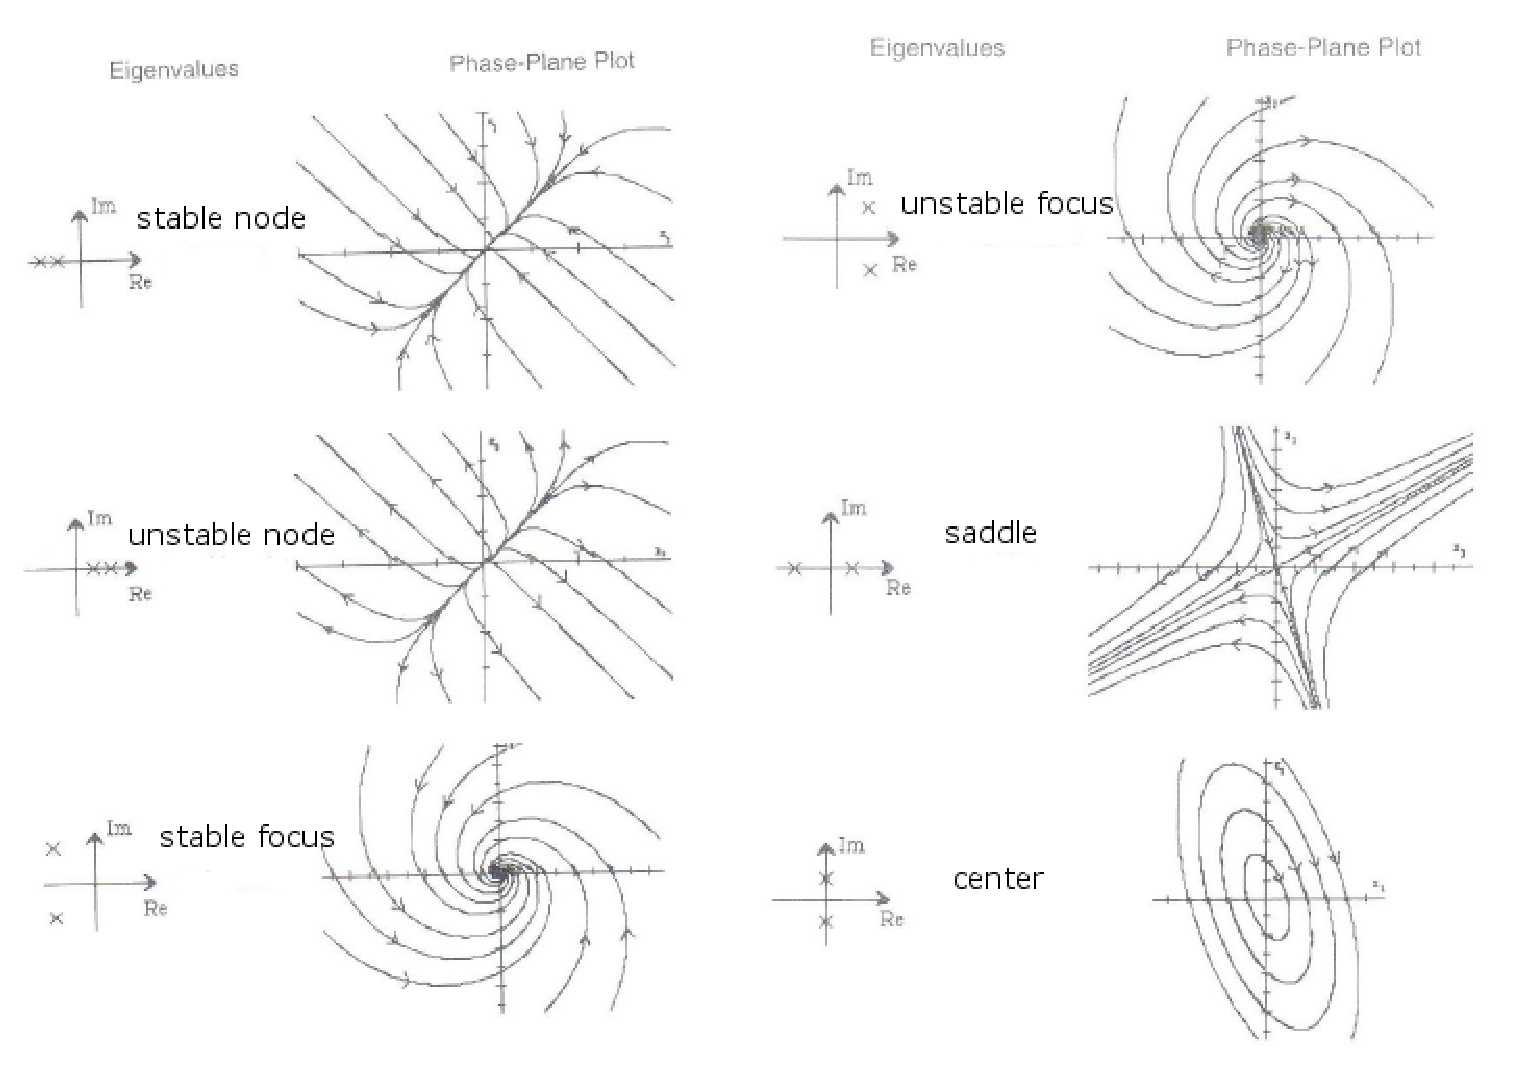
\includegraphics[height=8cm]{./images/phase-plane_eigenvalues.eps}}
  \caption{Phase-plane behavior as a function of eigenvalue location}\label{fig:phase-plane_behavior}
\end{figure}

Some authors refer to the region between the two nullclines as a {\bf
  funnel} which drains into the equilibrium point.

\subsection{Phase-plane analysis on 2D non-linear systems}
\label{sec:phase-plane-analysis-2}

Based on the fact that, at the area/region about the equilibrium
point, when the system is closed enough to the equilibrium points, the
behavior of the non-linear system is linearized. As a matter of fact,
non-linear systems will often have the same general local phase-plane
behavior as the linear models. However, there is still one
difference. In non-linear system, there is often multiple steady state
solutions.

To know at which steady state solution, the system will converge to,
e.g. determine the stable steady state, phase-plane analysis is a
perfect tool. 

{\bf Example 1}:

\begin{equation}
  \label{eq:109}
  \dot{u} = v(u+1)
  \dot{v} = u(v+3)
\end{equation}
There are two steady state (equilibrium) solutions
\begin{itemize}
\item the trivial one: $u_s=v_s=0$
\item the nontrivial one: $u_s=-1, v_s=-3$
\end{itemize}
This non-linear system can be linearized using the matrix
\begin{equation}
  \label{eq:110}
  A = \left[
    \begin{array}{cc}
      v_s & u_s + 1 \\
      v_x+3 & v_s 
    \end{array} 
    \right]
\end{equation}
and the linearized model is 
\begin{equation}
  \label{eq:112}
  \mathbf{\dot{x} = Ax}
\end{equation}
 $\mathbf{x=z-z_s}$ with $z=(u,v)'$ and $z_s = (u_s,v_s)'$.

\begin{itemize}
\item {\it Trivial solution}:
  \begin{equation}
    \label{eq:111}
  A = \left[
    \begin{array}{cc}
      0 &  1 \\
      3 & 0
    \end{array} 
    \right]    
  \end{equation}
  Finding the eigenvalues of this matrix: $\lambda_1 = -\sqrt{3},
  \lambda_2 = \sqrt{3}$. Then, the equilibrium point is a {\bf saddle point}.
\begin{figure}[htb]
  \centerline{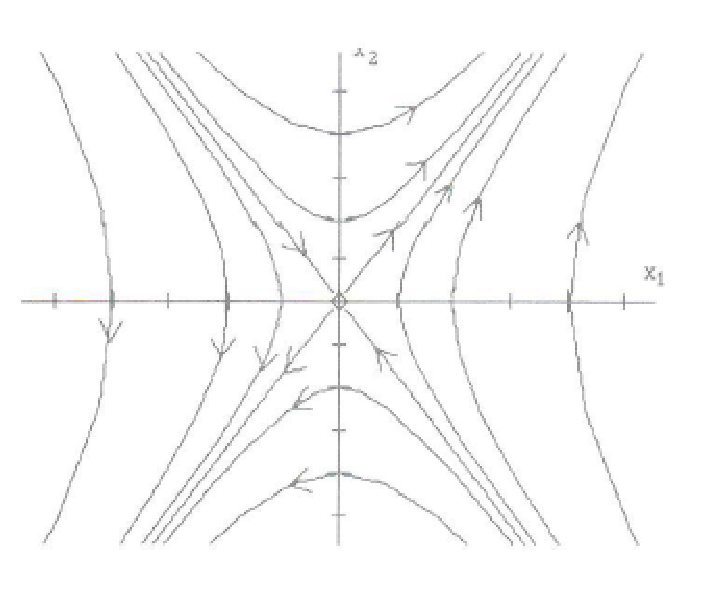
\includegraphics[height=5cm]{./images/saddle_nonlinear.eps}}
  \caption{Saddle point in a nonlinear system}\label{fig:saddle_nonlinear}
\end{figure}

\item {\it Non-trivial solution}:
  \begin{equation}
    \label{eq:1111}
  A = \left[
    \begin{array}{cc}
      -3 &  0 \\
      0 & -1
    \end{array} 
    \right]    
  \end{equation}
  Finding the eigenvalues of this matrix: $\lambda_1 = -3, \lambda_2 =
  -1$. Then, the equilibrium point is a {\bf stable} point. There is a
  ``fast'' stable eigenvector and a ``slow'' stable eigenvector.
\begin{figure}[htb]
  \centerline{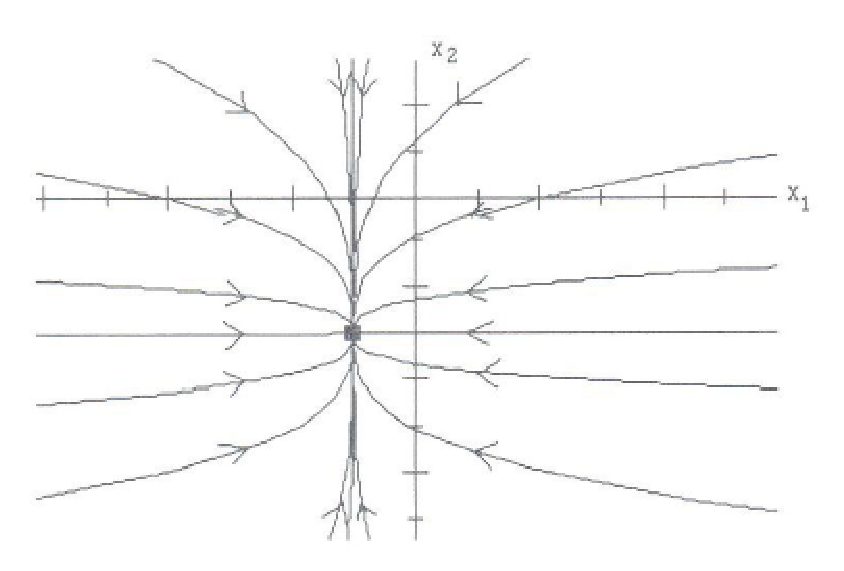
\includegraphics[height=5cm]{./images/stable_nonlinear.eps}}
  \caption{Stable point (stable node) in a nonlinear system}
  \label{fig:stable_nonlinear}
\end{figure}
\end{itemize}
Combining the two phase-plane, the fusion phase-plane for the
non-linear system is

\begin{figure}[htb]
  \centerline{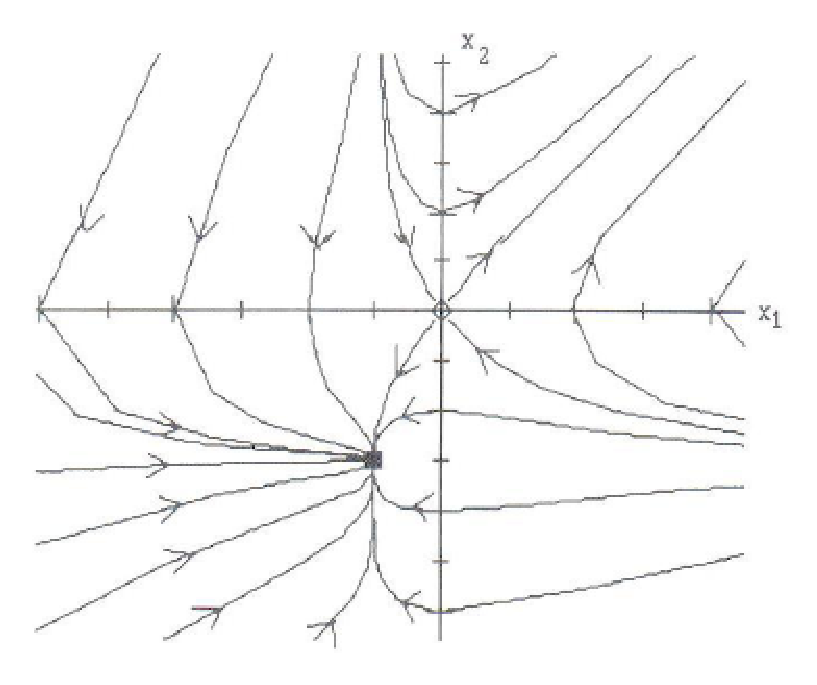
\includegraphics[height=5cm]{./images/phase-plane_nonlinear.eps}}
  \caption{The linearized model capture the behavior of a nonlinear
    model when close to equilibrium points. Here, the system has two
    critical points (filled circle: stable point, hollow circle: unstable
    point)}
\label{fig:phase-plane_nonlinear}
\end{figure}


\begin{lstlisting}[language=MatLab]
% Nonlinear Model
for h10 = 8 : 12
  for h20 = 4 : 8
    y0=[h10 h20];
    [t,y]=ode45('phaseplane', [0 200], y0);
    plot(y(:,1),y(:,2), y(1,1),y(1,2),'o'); hold on;
    xlabel('h_1'); ylabel('h_2');
    title('Phase-Plane Plot');
  end
end

% Linearized Model
for h10 = -2 : 2
  for h20 = -2:2
    y0=[h10 h20];
    [t,y]=ode45('phaseplane_L', [0 200], y0);
    y(:,1) = y(:,1)+10; 
    y(:,2) = y(:,2)+6;
    plot(y(:,1),y(:,2),'r', y(1,1),y(1,2),'o'); hold on;
  end
end

function dy = phaseplane(t,y)
  A1=5; A2=10; R1=2.5; R2=5/sqrt(6); F=5;
  dy(1) = F/A1-R1/A1*sqrt(y(1)-y(2));
  dy(2) = R1/A2*sqrt(y(1)-y(2))-R2/A2*sqrt(y(2));
  dy = dy';

function dy = phaseplane_L(t,y)
  A = [-0.125 0.125; 0.0625 -0.1042];
  dy = A*y;
\end{lstlisting}

\begin{figure}[htb]
  \centerline{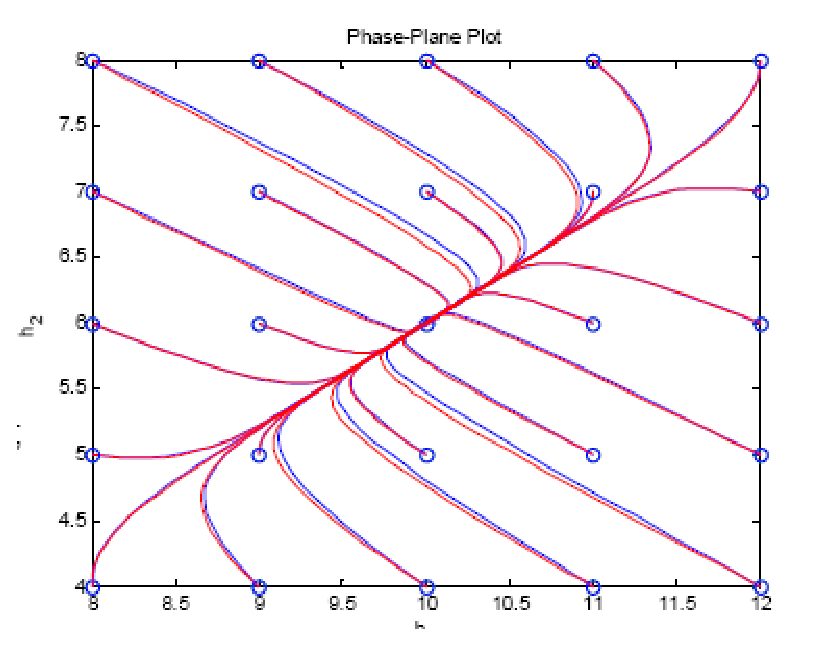
\includegraphics[height=5cm]{./images/phase-plane_plot.eps}}
  \caption{Phase-plane plot of the code. It's
  impossible to know the critical point is stable
  or unstable unless we add the arrows}
  \label{fig:phase-plane_plot}
\end{figure}


{\bf How can we find all fixed points using programming language?}:
E.g. $P=2r - 0.04rf; Q = -f + 0.01rf$
\begin{itemize}
\item {\it Mapple}:
\begin{verbatim}
restart;
P:= 2*r - 0.04 * r * f;
Q:= -f + 0.01 * r * f;
solve({P=0, Q=0}, {r,f});
----------------
       {r = 0.; f = 0.}, {r = 100.; f = 50.}
\end{verbatim}

\item {\it R statistic}:

\end{itemize}
Here, you have 2 stationary points. 

For a system that can be put into standard form, there are 4 types of
stationary points. 

\begin{figure}[htb]
  \centerline{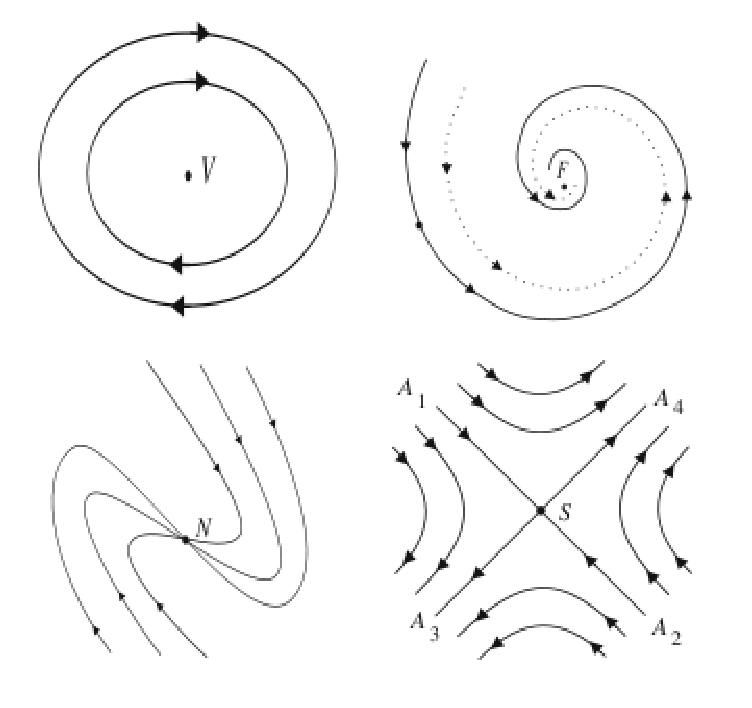
\includegraphics[height=5cm]{./images/stationary_points.eps}}
  \caption{Curves near stationary points: (V) vortex, (F) focal, (N)
    nodal, and (S) saddle point}\label{fig:stationary_points}
\end{figure}
With vortex (V), the curves oscillate indefinitely about the origin V
with no change in amplitude. A vortex point is surrounded by a
continuum of closed loop. 

With a spiral or focal point (F), the curves oscillate with an ever-decreasing
amplitude, asymptotically approaching the origin. as $t\rightarrow
\infty$. The focal point is called the {\it stable equilibrium
  point}. 

The saddle point is found as in the example of Romeo-Juliet model. 

\subsection{Predator-prey model}
\label{sec:predator-prey-model}
\label{sec:Lotka-Volterra-equation}

Ecologists try to understand the dynamics of species population in an
ecosystem. Here, a simple model with 2 species is taken as example:
one predator and one prey.

The {\bf Lotka-Volterra} equation (or Predator-Prey equation)
is the simplest and most widely used equation to model an oscillation system of
two variables (one representing population of prey and one representing
population of predator).

The model was developed independently by Lotka (1925) and Volterra (1926).
\begin{equation}
  \label{eq:82}
  \begin{split}
      \dot{X} = X(A-BY-\lambda X) \\
      \dot{Y} = Y(CX-D- \mu Y)
  \end{split}
\end{equation}
with $X(t), Y(t)$ is the population of the prey, and the predator,
respectively. A, B, C, D, $\mu$ and $\lambda$ are all positive
parameters of this dynamical system (the meaning of such parameters
are skipped here)\footnote{\url{http://home.comcast.net/~sharov/PopEcol/lec10/lotka.html}}. 
The condition for this problem is that $X\ge 0, Y\ge 0$.

The 3 potentially steady states are:
\begin{enumerate}
\item X = 0, Y = 0

\item X = A/$\lambda$, Y = 0

\item $X=\frac{\frac{A\mu}{B}+D}{C+\frac{\mu\lambda}{B}}$, 
$Y = \frac{\frac{CA}{\lambda} - D}{mu + \frac{BC}{A}}$
\end{enumerate}
since (X = 0, Y = -D/$\mu$) is not a legal steady state.

Given a position in the phase plan (X,Y), i.e. the population of both
the prey and predator. The question is, where in the phase plane the
population will move next. The phase plane, with the {\it directional
  arrows} can solve this.

Each point in the phase plane has 2 directional arrows associated
it. One horizontal arrow, either points to the left or right, tell
whether the prey population (X) is increasing or decreasing,
i.e. $\dot{X} > 0$ (right) or $\dot{X} < 0$ (left). Similar situation
is applied for the vertical arrow. Clearly, using such directional
arrows will tells us the trend of the population change. The core
question is how to determine which way my directional arrow points?
This is the tricky part.

In this example, the nullcline for X, i.e. $\dot{X}=0$, are all points
(X,Y) along this line
\begin{equation}
  \label{eq:100}
  X(A-BY-\lambda X) = 0
\end{equation}
As $B>0, Y\ge 0$, if Y increase, then the left side of
eq.~\eqref{eq:100} should decrease. Therefore, $\dot{X}<0$. In other
words, the directional arrow above $\dot{X}$ should point to the
left. And any directional arrow below $\dot{X}$ should point to the
right. 

\begin{enumerate}
\item Write the two ordinary differential equations 

\item Find and plot the nullclines

\item Label the isosectors, i.e. the spaces in the phase plane that
  are bordered by the nullclines, with I, II, III, etc.

\item In each isosector, find the two directional arrows (one should
  either up or down, and the other should either left or right)
  depending on the signs of $\dot{X}$ and $\dot{Y}$.

\item Draw a sample trajectory of the system (on the $u,v$-plane)
  through time, conforming to the directional arrows.
\end{enumerate}

\subsection{Spring oscillator}
\label{sec:spring-oscillator}

The oscillation of a mass $m$ attached to a light spring (spring
constant $k$) that obey Hooke's law with a friction force (with
damping coefficient $\gamma$) follows this equation
\begin{equation}
  \label{eq:102}
  \ddot{x} + 2\gamma \dot{x} + \omega^2 x = 0
\end{equation}
with $\omega=\sqrt{k/m}$ is the characteristic frequency. 

This second-order ODE can be transformed into the standard form with
$f(x,v) = \dot{x} = v, g(x,v) = \dot{v} = -2\gamma v + \omega^2 x$.

Then, the slope of the trajectory at any point $(x,v$) is
\begin{equation}
  \label{eq:104}
  \frac{dv}{dx} = \frac{-2\gamma v + \omega^2 x}{v}
\end{equation}

All of these behaviors are discussed in the next
Appendix ~\ref{chap:bifurcation-theory} (Bifurcation theory).

\subsection{Reduced a system for phase-plane analysis}
\label{sec:reduced-system-phase}

The example here is referred to as {\it Lindermann mechanism for
  gas-phase unimolecular reactions}. 
\begin{equation}
  \label{eq:113}
  \begin{split}
      \ce{A + A <=>[k_1][k_{-1}] A + B} \\
      \ce{B ->[k_2] P}
  \end{split}
\end{equation}
Here, A is the reactant, B is an energized molecule of A, and P is the
product.

To study the dynamics of the mechanism, a mathematical model is
formulated. According to the {\bf law mass action}, the
{\it rate of reactions} are

\begin{equation}
  \label{eq:114}
  \begin{split}
    \frac{d[A]}{dt} &= -k_1[A]^2 + k_{-1}[A][B] \\
    \frac{d[B]}{dt} &= k_1[A]^2 - k_{-1}[A][B] - k_2[B] \\
    \frac{d[P]}{dt} &= k_2[B] \\
  \end{split}
\end{equation}

This is a dynamical system with differential equations give the rule
for evolving this system. However, due the law of mass conservation,
then $[A]+[B]+[P]=[A_0]=$ constant.

\begin{equation}
  \label{eq:115}
  \frac{d[A]}{dt} + \frac{d[B]}{dt} + \frac{d[P]}{dt} = \frac{d}{dt}([A]+[B]+[P])
  = 0
\end{equation}

It means that the third quantity can be inferred from the other two.
Then, the minimum number of variables that is required to completely
describe the system is 2.  Since the product forming stage (the 2nd
reaction) is treated as irreversible, so you'd better keep the first
equation of reaction. In other words, P is eliminated to turn
eq.~\eqref{eq:114} to the standard form below.
\begin{equation}
  \label{eq:258}
    \begin{split}
    \frac{d[A]}{dt} &= -k_1[A]^2 + k_{-1}[A][B] \\
    \frac{d[B]}{dt} &= k_1[A]^2 - k_{-1}[A][B] - k_2[B] \\
  \end{split}
\end{equation}

In this problem, the two state variables [A] and [B] can have their
own units. To help analyzing the problem convenient, you should use
dimensionless variables. Convention:
{\it use lower-case letters for the dimensionless variables}
\begin{equation}
  \label{eq:117}
  a = k_1A/k_2; b = k_1B/k_2; \tau = k_2t
\end{equation}
with $\tau$ denotes for the time rate of change.  Then, the first
equation
\begin{equation}
  \label{eq:116}
  \begin{split}
    \frac{d\frac{k_2a}{k_1}}{d(\tau/k_2)} = -k_1 (\frac{k_2a}{k_1})^2
    + k_{-1} (\frac{k_2a}{k_1}) (\frac{k_2b}{k_1}) \\
\therefore* \frac{da}{d\tau} = -a^2 + \frac{k_{-1}}{k_1}ab
  \end{split}
\end{equation}
As $\alpha = k_{-1}/k_1$ is a dimensionless parameter, then
\begin{equation}
  \label{eq:118}
  \frac{da}{d\tau} = -a^2 + \alpha ab
\end{equation}
Similarly, the new form for the second equation
\begin{equation}
  \label{eq:119}
  \frac{db}{d\tau} = a^2 - \alpha ab - b
\end{equation}
Thus, you have
\begin{equation}
  \label{eq:120}
  \begin{split}
      \dot{a} = -a^2 + \alpha ab  \\
      \dot{b} = a^2 - \alpha ab - b
  \end{split}
\end{equation}



\subsection{Summary}
\label{sec:summary-5}

Here, phase plane does not tell us any specific numerical solutions; otherwise,
it does give a very good idea of how the system will behave over
time. Here is the summary of important concepts:
\begin{itemize}

\item {\bf phase plane} (state plane): the plane with two coordinates
  are two state variables

\item {\bf phase space}: if the system has three variables or more,
  state plane is now called phase space.

\item {\bf phase plane trajectory}: a curve on the phase plane
  corresponding to a specific initial condition

\item {\bf phase plane portrait}: plot of family of state
  trajectories, i.e. of the same system with different initial
  conditions.

\item {\bf phase plane plot}: a common name for phase plane
  trajectory, and phase plane portrait.


\item {\bf flow in phase plane}: the slope is the tangent of the angle
  which can be represented as
  \begin{equation}
    \label{eq:105}
    \frac{u'}{v'} = \frac{du}{dv} = \tan(\alpha) = \text{slope}
  \end{equation}
  Hence, the sign of the first-order derivative will tell the
  direction of the change. The slope, at a single point, can be
  denoted by an arrow (vector). The set of all arrows is called a
  {\bf vector-field} ({\it flow field},
  {\it tangent
    field}\footnote{as
    an arrow is tangent to the trajectory}).
  The flow field can provide a general idea of what all trajectories
  look like. From the starting point $(u(0),v(0))$, by following where
  these vectors lead you, you can obtain the trajectory. As a result,
  the phase-plane plot is filled with a grid of uniformly spaced
  arrows indicating the direction of increasing time and the slope at
  each point.

  % \item {\bf phase-plane portrait}: For a given set of initial
  %   condition, the subsequent temporal evolution of the system may be
  %   traced out by moving from one arrow to the next and drawing an
  %   appropriate line (curve) for the trajectory. Pictures containing
  %   vector field  are called {\it phase-plane portraits}.

  %   The question is ``how many vectors is enough''? - it is a
  %   common choice to draw the vectors at the steady states.

  %   To know the time
  %   evolution of the system, one can draw arrows connecting every two
  %   points of consecutive time instants, e.g. $(u(0),v(0)) \rightarrow
  %   (u(t_1),v(t_1)), (u(t_1),v(t_1))\rightarrow (u(t_2),v(t_2))$. This set
  %   of arrows (vectors) is called a vector-field.


\item {\bf steady state} (fixed point) : there are some points where
  the system does not evolve in time, e.g. $u'=0$ or $v'=0$. The pair
  of (u,v) at a time instant, such that the two first-order
  derivatives are zero is called {\bf steady state} or fixed
  point. So, if you start from a fixed point, thing will never
  change. The interesting question is what if you start from a point
  close to the fixed point. The system can either return to the fixed
  point or moving away from this closed fixed point. Such closed fixed
  point is called stable fixed point in the former case and is called
  an unstable fixed point in the latter case.  This will be discussed
  more details in the next
  \hyperref[sec:phase-plane-analysis-1]{section}.
  % This will be discussed
  % more details in the next \hyperref[sec:steady-stat-isocl]{section}.

\item {\bf stationary point}: The input, e.g. ($u,v$), of a function
  where the first-order derivative, e.g. $f(u,v)$, is zero is called
  {\it stationary point}. Otherwise, the input is called
  {\it ordinary point}.

\end{itemize}

% \subsection{Steady states and isoclines}
% \label{sec:steady-stat-isocl}

\section{Manifolds}

Manifolds of a dimension $n$ is a topological space near a 
$n$-dimensional point, that can resememble the $n$-dimensional Euclidean space.
So, instead of studying the system at a vast space, we just focus on the
variation of the variable in the manifold around a certain point. 

At first, we use eigenvalues method to classify the critical points
$\mathbf{x}^*$ (saddle, (stable/unstable) focus, center, (stable/unstable)
node). A stable manifold of a critical point $\mathbf{x}^*$, is defined as the
set of initial conditions such that $\mathbf{x}(t)\rightarrow \mathbf{x}^*$ as
$t\rightarrow \infty$. An unstable manifold of a critical point $\mathbf{x}^*$,
is defined as the set of initial conditions such that $\mathbf{x}(t)\rightarrow
\mathbf{x}^*$ as $t\rightarrow -\infty$.


A critical point $\mathbf{x}^*$ is {\bf atracting} if there is a small enough
distance $\delta > 0$, and whenever we start with an initial condition $\mathbf{x}(0)$
such that $||\mathbf{x}(0)-\mathbf{x}^*|| < \delta$, then the system converge to
$\mathbf{x}^*$. 

A critical point $\mathbf{x}^*$ is {\bf globally atracting} if for all initial
condition $\mathbf{x}(0)$, the system converge to $\mathbf{x}^*$.

A critical point $\mathbf{x}^*$ is {\bf Liapunov stable} for each $\epsilon >0$,
there is always existing a small enough distance $\delta > 0$, so that all
initial condition within that manifold,  and $||\mathbf{x}(t)-\mathbf{x}^*|| <
\epsilon$ whenever $t\ge 0$.

A critical point $\mathbf{x}^*$ is {\bf asymptotic stable} if it's both {\it
attracting} and {\it Liapunov stable}. 

\section{Tools for phase plane analysis}
\label{sec:tools-phase-plane}


\subsection{XPPAUT}
\label{sec:case-study-10-1}

Consider the FitzHugh-Nagumo model with two dependent quantities X, Y.

\lstinputlisting{./codes/XPPAUT/FHN_model.ode}

To perform phase-plane analysis, you can either do on the current
figure or create a new one. Set up the coordinate information with X
is x-axis, Y is y-axis, and the scales (range). If you don't know the
scale, just leave the default value and you can adjust it later
\underline{Window}-\underline{Fit} (key: WF). 

Adjust the scale (key: V2) x-axis as -0.5 to 1.5, and y-axis as -0.2
to 0.8. To add a nullclines, click
\underline{Nullcline}-\underline{New} (key: NN). The accuracy with
which the nullclines are computed is controlled by the nullcline mesh
(click \underline{nUmerics}-\underline{Ncln control} (key: UN). By
default, nullcline mesh is 40, you can try it with 100.

Steady states and associated eigenvalues can be computed using
\underline{Sing pts}-\underline{Go} and the values are printed on the
X-window. If there are more than one steady states, use
\underline{Sing pts}-\underline{Mouse} to zero in on a particular
steady state. 

Experience with \underline{Initialconds}-\underline{Mouse} command and
then redraw nullclines (key: NN).


\subsection{DFIELD and PPlane}
\label{sec:dfield-pplane}

It has Matlab version and Java version.


References:
\begin{itemize}
\item \url{http://math.rice.edu/~dfield/index.html}
\item \url{http://math.rice.edu/~dfield/dfpp.html}
\item \url{http://controls.engin.umich.edu/wiki/index.php/PhasePlaneAnalysis}
\end{itemize}

\subsection{Mathematica}
\label{sec:mathematica}

Consider a system:
\begin{equation}
  \label{eq:654}
  \begin{split}
    \dot{x} = x + y \\
    \dot{y} = -4x + y
  \end{split}
\end{equation}

To plot vector field, we use
\begin{lstlisting}
Needs["Graphics `PlotField`"]

PlotVectorField[{ x+y, -4*x+y}, {x, -3,3 }, 
  { y,-3,3}, Axes -> True, Ticks -> None, 
  Frame -> True, AspectRatio -> 1] 
\end{lstlisting}
TO scale the vector to unit length, we can add this to the square
bracket
\begin{verbatim}
ScaleFunction ->(1&) 
\end{verbatim}

\subsection{Matlab - Matcont}
\label{sec:matlab}

\hyperlink{http://www.matcont.ugent.be/}{Matcont} is a package written
in MatLab.  Consider a system:
\begin{equation}
  \label{eq:654}
  \begin{split}
    \dot{x} = x + y \\
    \dot{y} = -4x + y
  \end{split}
\end{equation}

To plot vector field, we use
\begin{lstlisting}
[x,y]=meshgrid(-3:0.475: 3, -3:0.475:3);

z1=x+y;

z2=-4*x+y;

quiver(x,y,z1,z2)

grid 
\end{lstlisting}


% \section{Phase space}
% \label{sec:phase-space}

% A system with $n$ degree of freedoms (DOFs - the number of state
% variables) requires $n$ positional data $q_1...q_n$ for it location to
% be completely determined. However, the state of the system at time $t$
% is fully determined given the values of $q_i(t)$ and the corresponding
% velocities $\dot{q_i}(t)$, $i=\overline{1..n}$. In total, we need $2n$
% quantities. Thus, we may consider
% $(q_1,\dot{q_1},q_2,\dot{q_2},...q_n,\dot{q_n})$ (written as
% $q_i(t),\dot{q_i}(t)$ for short) as a point in a $2n$ dimensional space
% called {\bf phase space}. 

% For any given initial condition $q_i(0),\dot{q_i}(0)$, it corresponds
% to a point $M_0$ in the phase space; then when the time $t$ varies,
% from the point $M_0$ it draw a curve called {\bf path} (or
% {\bf trajectory}), which describes the history of the system.  Each
% point $M$ is called the {\bf phase point} which is identical to a
% particular state of the system.


% The figure that containing all {\it paths} of a single system is
% called a {\bf phase portrait} of the system. It represents all
% possible histories of the system. Each path correspond to a given
% initial condition, or the single state $M_0$. It means that
% \textcolor{red}{on the phase space, there is one and only one path
%   through each point},
% except singular points that has all paths going through it.


%%% Local Variables: 
%%% mode: latex
%%% TeX-master: "mainfile"
%%% End: 
